\documentclass[a4paper, 12pt]{article}
\usepackage[utf8]{inputenc}
\usepackage[portuguese]{babel}
\usepackage{amsmath, amsthm, amssymb}
\usepackage[hidelinks]{hyperref}
\usepackage{enumerate}
\usepackage{graphicx}
\usepackage{indentfirst}
\usepackage[sorting=none]{biblatex}
\usepackage{pythonhighlight}
\usepackage{float}

\graphicspath{{./imagens/}}
\addbibresource{bibliography.bib}

\title{Trabalho 2 - Relatório}
\author{Carolina Dias}
\date{June 2022}

\newtheorem{teorema}{Teorema}
\newtheorem{lema}{Lema}
\newtheorem{corolario}{Corolário}
\newtheorem{proposicao}{Proposição}
\theoremstyle{definition}
\newtheorem{definicao}{Definição}
\newtheorem{questao}{}
\newtheorem{exemplo}{Exemplo}
\newtheorem{notation}{notação}

\newenvironment{solucao}{\noindent\textbf{Solução.}}{}
\newenvironment{demonstracao}{\noindent\textit{Demonstração.}}{\qed}
	
\theoremstyle{remark}
\newtheorem{observacao}{Observação}
%\includeversion{resposta}

\makeindex
	
\begin{document}

\begin{titlepage}
	\begin{center}
	    
\includegraphics[width=1.5cm]{logo-uece}\\
		\textsc{Universidade Estadual do Ceará\\Centro de Ciências e Tecnologia\\Programa de Pós-Graduação em Ciência da Computação\\Mestrado Acadêmico Em Ciência Da Computação}
		
		\vspace{5cm}
		{\small {\textsc Relatório Técnico II}}
		
		\vspace{1cm}
		
		{\huge Classificação: \textit{Concrete Crack Images for Classification}}
		
		\vspace{1cm}
		\textbf{Carolina Araújo Dias}
		
		\vspace{6.5cm}
		Junho de 2022
		
	\end{center}
\end{titlepage}

\begin{center}
    \section*{Resumo}
\end{center}

Neste trabalho utilizamos conceitos de redução de dimensionalidade para resolvermos um problema de classificação da existência de rachaduras em imagens de concreto. Utilizamos inicialmente a Decomposição Espectral de matrizes, seguida pela Decomposição em Valores Singulares (SVD). Com isso reduzimos a quantidade de características dos dados, que, originalmente, são 1024. Foi utilizado o algoritmo de classificação do vizinho mais próximo KNN com k = 1 e obtidos resultados satisfatórios para a acurácia. Conseguimos obter, ao utilizar a SVD, uma acurácia de $95,77\%$ para os dados de teste utilizando apenas 17 das 1024 características.

\textbf{Palavras-chave:} classificação, decomposição, svd. 


\newpage

\tableofcontents

\newpage

\section{Introdução}

Atualmente é bastante comum notarmos a necessidade de classificar de imagens automaticamente, utilizando algoritmos de aprendizado de máquina. No cenário deste trabalho, realizar a classificação da existência de rachaduras em concreto é de grande utilidade para detectá-las sem a intervenção humana, economizando tempo e dinheiro.

Entender a Álgebra Linear que há por trás desse processo é uma etapa bem recompensadora, pois transforma a "caixa preta" em algo simples, belo e tangível.

Assim, veremos como realizar a redução de dimensionalidade de dados utilizando duas técnicas, a Decomposição Espectral e a Decomposição em Valores Singulares. Com isso, obtemos resultados bastante satisfatórios utilizando apenas uma parcela dos dados, economizando em poder de processamento e até mesmo no entendimento geral.

\newpage
\section{Trabalhos Relacionados}

Classificar imagens é um tema amplamente estudado. Para o conjunto de dados em questão, o \textit{Concrete Crack Images for Classification}, dois trabalhos se destacam na utilização do mesmo, mas com técnicas que vão além das utilizadas neste trabalho. Mesmo assim, o conceito se mantém.

Em \cite{ozgenel2018} a classificação das imagens de concreto foi realizada através de redes neurais pré-treinadas e suas performances foram comparadas. Esse resultado é importante para o uso em inspeções de prédios e imóveis, mas se mostra um desafio quando observadas as imagens do "mundo real", pois nem sempre a qualidade destas está à altura das imagens utilizadas em experimentações fechadas, como as que utilizamos aqui.

Já em \cite{zhang2016}, o problema e conjunto de dados em questão foi adaptado para a detecção de rachaduras em rodovias, uma aplicação também bastante importante para a manutenção de ruas e estradas. As imagens foram utilizadas para treinar uma rede neural convolucional e seus resultados se mostraram superiores a outros métodos de classificação da existência de rachaduras nesse conjunto de dados.

Mesmo que não sejam utilizadas técnicas como redes neurais, é possível obter um bom valor de acurácia para esse problema utilizando de técnicas advindas da Álgebra Linear, como faremos a seguir.

\newpage
\section{Fundamentação Teórica}

Com o objetivo de realizarmos uma classificação, podemos simplesmente aplicar um algoritmo pré-pronto sem entender o que há por trás do código e obter um resultado bom o suficiente. Mas para irmos além e entender a fundo como ocorre uma classificação, podemos usar técnicas como redução de dimensionalidade, bastante útil quando utilizamos imagens no processo, pois estas possuem uma grande quantidade de características.

Com isso em mente, vamos entender como funciona a redução de dimensionalidade utilizando tanto a decomposição espectral de uma matriz quanto a decomposição em valores singulares (SVD).

\subsection{Decomposição Espectral}

Para entendermos como realizar a decomposição espectral de uma matriz precisamos entender o conceito de diagonalização.

\begin{definicao}
    Duas matrizes $A$ e $T$ são \textit{similares} se existir uma matriz invertível $S$ tal que $$A = STS^{-1}.$$
\end{definicao}

Se restringirmos a matriz $T$ a ser uma matriz diagonal, então temos o conceito de \textit{matriz diagonalizável}.

\begin{definicao}
    Uma matriz será dita \textit{diagonalizável}, se ela for similar a uma matriz diagonal.
\end{definicao}

Com essas definições, conseguimos entender melhor o

\begin{teorema}
    Se uma matriz $A$ $n \times n$ possuir $n$ autovetores linearmente independentes, então $A$ será diagonalizável. A decomposição $$A = S\Lambda S^{-1}$$ é chamada de decomposição espectral (ou de autovalor) da matriz $A$, sendo $\Lambda$ uma matriz diagonal com os autovalores de $A$ em sua diagonal principal.
\end{teorema}

\begin{demonstracao}
    Suponha que $A$ tem $n$ autovetores linearmente independente $x_1, \ldots, x_n$, associados aos autovalores $\lambda_1, \ldots, \lambda_n$, não necessariamente distintos. Agora formamos a matriz $S$ tal que
    $$S =
    \begin{bmatrix}
    \vert & \vert & \  & \vert \\
    \mathbf{x_1} & \mathbf{x_2} & \dots & \mathbf{x_n} \\
    \vert & \vert & \ & \vert
\end{bmatrix}.$$

Então vale que $S$ é invertível e

\begin{align*}
AS &= A
\begin{bmatrix}
    \vert & \vert & \  & \vert \\
    \mathbf{x_1} & \mathbf{x_2} & \dots & \mathbf{x_n} \\
    \vert & \vert & \ & \vert
\end{bmatrix}
=
\begin{bmatrix}
    \vert & \vert & \  & \vert \\
    A\mathbf{x_1} & A\mathbf{x_2} & \dots & A\mathbf{x_n} \\
    \vert & \vert & \ & \vert
\end{bmatrix}
=\\
&=
\begin{bmatrix}
    \vert & \vert & \  & \vert \\
    \lambda_1 \mathbf{x_1} & \lambda_2 \mathbf{x_2} & \dots & \lambda_n \mathbf{x_n} \\
    \vert & \vert & \ & \vert
\end{bmatrix}
=
\begin{bmatrix}
    \vert & \vert & \  & \vert \\
    \mathbf{x_1} & \mathbf{x_2} & \dots & \mathbf{x_n} \\
    \vert & \vert & \vert
\end{bmatrix}
\begin{bmatrix}
    \lambda_1 & \dots  & 0\\
    \vdots & \ddots & \vdots\\
    0 & \dots & \lambda_n
\end{bmatrix}
\Leftrightarrow\\
&\Leftrightarrow AS = SD \Leftrightarrow A = SDS^{-1}.
\end{align*}

Com isso, $A$ é semelhante a $D$, que é diagonal, logo $A$ é diagonalizável.

\end{demonstracao}

Para utilizarmos a decomposição espectral para a redução de dimensionalidade, precisamos calcular a decomposição para a matriz de covariância dos dados, ao invés da matriz original $A$:

$$m \times cov(A) = m \frac{1}{m}X^TX = X^TX = Q\Lambda Q^T.$$

Após, ordenamos seus autovalores em ordem decrescente $$\lambda_1 \geq \lambda_2 \geq \dots \geq \lambda_n \geq 0,$$ e calculamos a variabilidade acumulada

$$E(r) = \frac{\lambda_1 + \lambda_2 + \dots + \lambda_r}{\lambda_1 + \lambda_2 + \dots + \lambda_n}.$$

Aqui nos resta escolher qual $r$ representa um bom compromisso entre uma alta variabilidade acumulada e um pequeno valor para $r$. Encontrado esse $r$ satisfatório, calculamos a matriz $\hat{Q}$ com as primeiras $r$ colunas de $Q$. Finalmente, conseguimos encontrar as componentes principais da matriz original $A$

$$\hat{A} = A\hat{Q}.$$

Essa nova matriz $\hat{A}$ representa uma redução de dimensionalidade da matriz $A$, sem comprometer os resultados obtidos pela mesma. Ou seja, podemos aplicar algoritmos de classificação, como o k vizinhos mais próximos (KNN) e mesmo assim não ter grandes perdas em sua acurácia ao utilizarmos apenas uma fatia dos dados, calculada acima.

\subsection{Decomposição em Valores Singulares (SVD)}

Agora voltamos o olhar para a Decomposição em Valores Singulares (SVD, na sigla em inglês) que também é amplamente utilizada para realizar a redução de dimensionalidade dos dados. Vejamos como funciona a Decomposição em Valores Singulares Reduzida, pois a utilizamos na nossa base de dados. Aqui queremos encontrar uma decomposição da forma

$$X = \hat{U}\hat{S}V^T$$

tal que

\begin{itemize}
    \item $\hat{U}$ é uma matriz $m \times n$, com colunas ortonormais, chamadas \textbf{vetores singulares esquerdos} de $X$;
    \item $\hat{S}$ é uma matriz $n \times n$ diagonal, onde seus elementos da diagonal principal são os \textbf{valores singulares} de $X$;
    \item $V$ é uma matriz $n \times n$ ortogonal, cujas colunas são os \textbf{vetores singulares direitos} de $X$ e representam os autovetores de $X^TX$.
\end{itemize}

Também vale que

\begin{equation*}
\hat{S} = 
\begin{bmatrix}
    \sigma_1 & \dots & 0 \\
    \vdots & \ddots & \vdots \\
    0 & \dots & \sigma_n
\end{bmatrix}
=
\begin{bmatrix}
    \sqrt{\lambda_1} & \dots & 0 \\
    \vdots & \ddots & \vdots \\
    0 & \dots & \sqrt{\lambda_n}
\end{bmatrix}
\end{equation*}

com $\sigma_1 \geq \sigma_2 \geq \dots \geq \sigma_n \geq 0$.

Com isso, conseguimos realizar a redução de dimensionalidade dos dados similarmente como fizemos no caso da decomposição espectral.

Após encontrarmos qual o melhor valor de $r$ para os dados em questão, através do cálculo da variabilidade acumulada, obtemos a matriz $\hat{V}$ formada pelas $r$ primeiras colunas de $V$. Assim, encontramos as componentes principais da matriz $X$ fazendo $$\hat{P} = X\hat{V}.$$

Novamente, com essa "fatia" dos dados, realizamos a classificação dos mesmos, sem grandes perdas no resultado se comparados a utilização de todas as características dos dados originais.

\subsection{Questões}

\begin{questao}
    Consideremos $Z$ a matriz $m \times n$ em cujas linhas estão as coordenadas das amostras em relação à \textbf{base de autovetores}, isto é:
    
    $$X^T = QZ^T.$$
    
    Mostre que
    
    $$Z = XQ.$$
\end{questao}

\begin{solucao}
\begin{align*}
X^T &= QZ^T \\
Q^TX^T &= Q^TQZ^T\\
Q^TX^T &= Z^T\\
(Z^T)^T &= (Q^TX^T)^T\\
Z &= XQ
\end{align*}

\end{solucao}

\begin{questao}
    Consideremos a equação $X^T = QZ^T$ e $\hat{Q}$ a matriz $n \times r$, com $r < n$, cujas colunas são as $r$ primeiras colunas de $Q$. \textbf{Definimos} a matriz $\hat{Z}$ $m \times r$ por:
    
    $$\hat{Z} = X\hat{Q}.$$
    
    Verificar numericamente, para o respectivo banco de dados, que
    
    $$\hat{Z} = Z[:, 0:r],$$
    
    isto é, que as colunas de $\hat{Z}$ são as $r$ primeiras colunas de $Z$.
\end{questao}

\begin{solucao}
 Utilizando o comando \pyth{np.allclose(Z_train, Z[:, :r])}, que compara as duas matrizes, obtemos o resultado \pyth{True}, o que nos diz que elas são sim iguais e que as colunas de $\hat{Z}$ (nesse caso \textit{Z\_train}) são as $r$ primeiras colunas de $Z$.
\end{solucao}

\begin{questao}
    Seguindo a equação $X^T = QZ^T$, \textbf{definimos} a matriz dos dados projetados por:
    
    $$\hat{X}^T = \hat{Q}\hat{Z}^T.$$
    
    Mostrar que os dados projetados são calculados pela equação
    
    $$\hat{X} = X\hat{Q}\hat{Q}^T.$$
\end{questao}

\begin{solucao}
\begin{align*}
X^T &= QZ^T \\
X &= ZQ^T\\
\hat{X}^TX &= \hat{X}^TZQ^T\\
\hat{Q}\hat{Z}^TX &= \hat{X}^TZQ^T\\
(\hat{X}^TZQ^T)^T &= (\hat{Q}\hat{Z}^TX)^T\\
QZ^T\hat{X} &= X^T\hat{Z}\hat{Q}^T\\
Q(Q^TX^T)\hat{X} &= X^T\hat{Z}\hat{Q}^T\\
X^T\hat{X} &= X^T\hat{Z}\hat{Q}^T\\
X^T\hat{X} &= X^TX\hat{Q}\hat{Q}^T\\
X^T\hat{X} &= \hat{Q}\hat{Q}^T\\
XX^T\hat{X} &= X\hat{Q}\hat{Q}^T\\
\hat{X} &= X\hat{Q}\hat{Q}^T
\end{align*}
\end{solucao}

\begin{questao}
    Mostrar que a matriz $\hat{Q}\hat{Q}^T$ é um \textbf{projetor ortogonal}.
\end{questao}

\begin{solucao}
    Para $\hat{Q}\hat{Q}^T$ ser um projetor ortogonal, deve valer $(\hat{Q}\hat{Q}^T)^2 = \hat{Q}\hat{Q}^T$ e $(\hat{Q}\hat{Q}^T)^T = \hat{Q}\hat{Q}^T$.
    
    Para a primeira condição:
    
    $$(\hat{Q}\hat{Q}^T)^2 = (\hat{Q}\hat{Q}^T)(\hat{Q}\hat{Q}^T) = \hat{Q}(\hat{Q}^T\hat{Q})\hat{Q}^T = \hat{Q}I\hat{Q}^T = \hat{Q}\hat{Q}^T.$$
    
    Para a segunda:
    
    $$(\hat{Q}\hat{Q}^T)^T = (\hat{Q}^T)^T(
    \hat{Q})^T = \hat{Q}\hat{Q}^T.$$
\end{solucao}

\begin{questao}
    Verificar numericamente, para o respectivo banco de dados, que
    
    $$\hat{Q}\hat{Q}^T \not\approx I.$$
\end{questao}

\begin{solucao}
 Utilizando o comando \pyth{np.allclose(np.matmul(Q_r, Q_r.T), np.identity(Q_r.shape[0]))}, que compara a matriz $\hat{Q}\hat{Q}^T$ com a identidade de mesmas dimensões, obtemos o resultado \pyth{False}, ou seja, elas não são iguais.
\end{solucao}

\begin{questao}
    Considerando uma matriz de dados centralizados $X$ $m \times n$, mostrar que as matrizes $X^TX$ e $XX^T$ possuem os mesmos autovalores não-nulos.
\end{questao}

\begin{solucao}
    Seja $\lambda$ um autovetor não-nulo de $X^TX$ e seu vetor associado $a$. Vale que
    
    \begin{align*}
        X^TXa &= \lambda a\\
        XX^TXa &= X\lambda a\\
        XX^T(Xa) &= \lambda (Xa)\\
        XX^T\tilde{a} &= \lambda \tilde{a}
    \end{align*}
    
Com isso, $\lambda$ é um autovalor de $XX^T$, associado ao vetor $\tilde{a} = Xa$.
\end{solucao}

\begin{questao}
    Verificar numericamente para a proposição anterior, calculando, para o respectivo banco de dados, os autovalores de $X^TX$ e $XX^T$.
\end{questao}

\begin{solucao}
    Primeiro encontramos as matrizes $X^TX$ e $XX^T$ e seus autovalores. Para comparar seus autovalores, precisamos selecionar apenas os autovalores não-nulos de $XX^T$. Isso foi feito com o comando \pyth{autovalores_XXT[autovalores_XXT>(1e-5)]}. Finalmente, os autovalores foram comparados com o comando\\\pyth{np.allclose(autovalores_XTX, autovalores_XXT_maiores_que_zero)}\\e o resultado foi o esperado, \pyth{True}.
\end{solucao}

\begin{questao}
    Considerando a SVD completa $X = USV^T$, mostrar que as colunas de $V$ são autovetores de $X^TX$ e que as $n$ colunas de $U$ são os autovetores de $XX^T$ associados aos $n$ maiores autovalores.
\end{questao}

\begin{solucao}
    Vimos que, na SVD, vale $V = Q$, onde $Q$ vem da decomposição espectral. E na decomposição espectral, as colunas de 
    $Q$ são autovetores de $X^TX$, ou seja,
    
    $$X^TX = (USV^T)^T(USV^T) = VS^TU^TUSV^T = VS^TSV^T.$$
    
    Daí, $V$ é a matriz de autovetores de $X^TX$. E $S^TS$ é a matriz de autovalores de $X^TX$.
    
    Agora,
    
    $$XX^T = (USV^T)(USV^T)^T = USV^TVS^TU^T = USS^TU^T.$$
    
    Daí, $U$ é a matriz de autovetores de $XX^T$. E $SS^T$ é a matriz de autovalores de $XX^T$.
\end{solucao}

\begin{questao}
    Verificar a proposição anterior, comparando, para o respectivo banco de dados, a matriz de autovetores de $X^TX$ e a matriz de vetores singulares direitos, isto é, $V$ em $X = USV^T$. Atenção para com os sentidos dos vetores.
\end{questao}

\begin{solucao}
    Calculamos os autovetores de $X^TX$ e encontramos $V$ na SVD completa. Porém, ao compararmos os valores com o comando \pyth{np.allclose(autovetores_XTX, V)} recebemos o resultado \pyth{False}. Também foi comparado com $V^T$, caso os sentidos dos vetores não estivessem coerentes. Aqui, também, obtemos \pyth{False} como resposta. Isso pode se dar ao fator de ocorrerem arredondamentos nos valores calculados, impedindo que eles se igualem, nesse caso.
\end{solucao}

\newpage
\section{Metodologia}

Para a realização da classificação de imagens com redução de dimensionalidade foi utilizada a linguagem \textit{Python}, versão 3.8.10, em um \textit{Jupyter Notebook}. Foram utilizadas bibliotecas que auxiliam na manipulação de dados e cálculos da Álgebra Linear, como \textit{NumPy} e \textit{Pandas}, e bibliotecas de visualização de dados, como a \textit{Matplotlib}. Além disso, a biblioteca \textit{Pillow} foi responsável pela manipulação de imagens. Por fim, foram utilizadas diversas funções da biblioteca de aprendizado de máquina \textit{Scikit-Learn}, tanto para realizar a classificação em si, com o método do vizinho mais próximo (KNN) como para a medição da acurácia dos resultados obtidos.

O conjunto de dados utilizado neste trabalho está relacionado à classificação da existência de rachaduras em concreto (\textit{Concrete Crack Images for Classification}).\cite{dataset} Existem 40.000 imagens de concreto, 20.000 com rachaduras (\textit{positive}) e 20.000 sem rachaduras (\textit{negative}).

Para melhor uso do conjunto de dados, foi realizado o pré-processamento das imagens. Para isso, para cada uma das imagens das duas classes \textit{Positive} e \textit{Negative}, foi realizado redimensionamento para $32 \times 32$ pixels. Além disso, foram convertidas de RGB para níveis de cinza (monocromáticas), com as funções \textit{Python} apropriadas: \pyth{.resize((32, 32)} e \pyth{.convert("L")}, ambas da biblioteca \textit{Pillow.}

Assim, cada uma das imagens foi salva em um vetor do \textit{NumPy} de tamanho $32 \times 32 = 1024$. Obtemos, então, uma matriz com 20.000 observações e 1024 características para cada uma das classes, 40.000 no total. Salvamos essa matriz em um \textit{DataFrame} do \textit{Pandas} para ser utilizado nos cálculos seguintes. Essa manipulação dos dados pode ser encontrada no \textit{notebook} \pyth{t02_data_manipulation.ipynb}.

Agora podemos realizar os passos necessários para a redução de dimensionalidade, para utilizarmos apenas uma fração das 1024 características e mesmo assim não termos perda de acurácia na classificação final.

\newpage
\section{Experimentos e Resultados}

\subsection{Decomposição Espectral}

Após convertemos as imagens para uma tabela, separamos os dados em dados de treinamento e dados de teste. Ficamos, assim, com 4 matrizes: \textit{X\_train, y\_train, X\_test, y\_test}.

Então, as matrizes \textit{X\_train} e \textit{X\_test} foram centralizadas. Após, foi calculada a matriz de covariância dos dados de treino \textit{X\_train} com o comando \pyth{np.cov(X_train, rowvar=False)}. Aqui o parâmetro \pyth{rowvar} deve ser setado como \pyth{False} pois as variáveis estão nas colunas e as observações estão nas linhas, como pode ser compreendido na documentação da biblioteca \textit{NumPy}.

Com a covariância, calculamos sua decomposição espectral com o comando \pyth{np.linalg.eigh(cov_treino)}. Isso nos retorna duas matrizes:\\ \pyth{autovalores_cov_treino} e \pyth{autovetores_cov_treino}. Os autovalores na matriz \pyth{autovalores_cov_treino} já vêm ordenados em ordem crescente, então basta invertê-los para que fiquem em ordem decrescente. Analogamente para \pyth{autovetores_cov_treino}.

Geramos então o gráfico da variabilidade acumulada por número de autovalores e obtemos:

\begin{figure}[H]
  \centering
  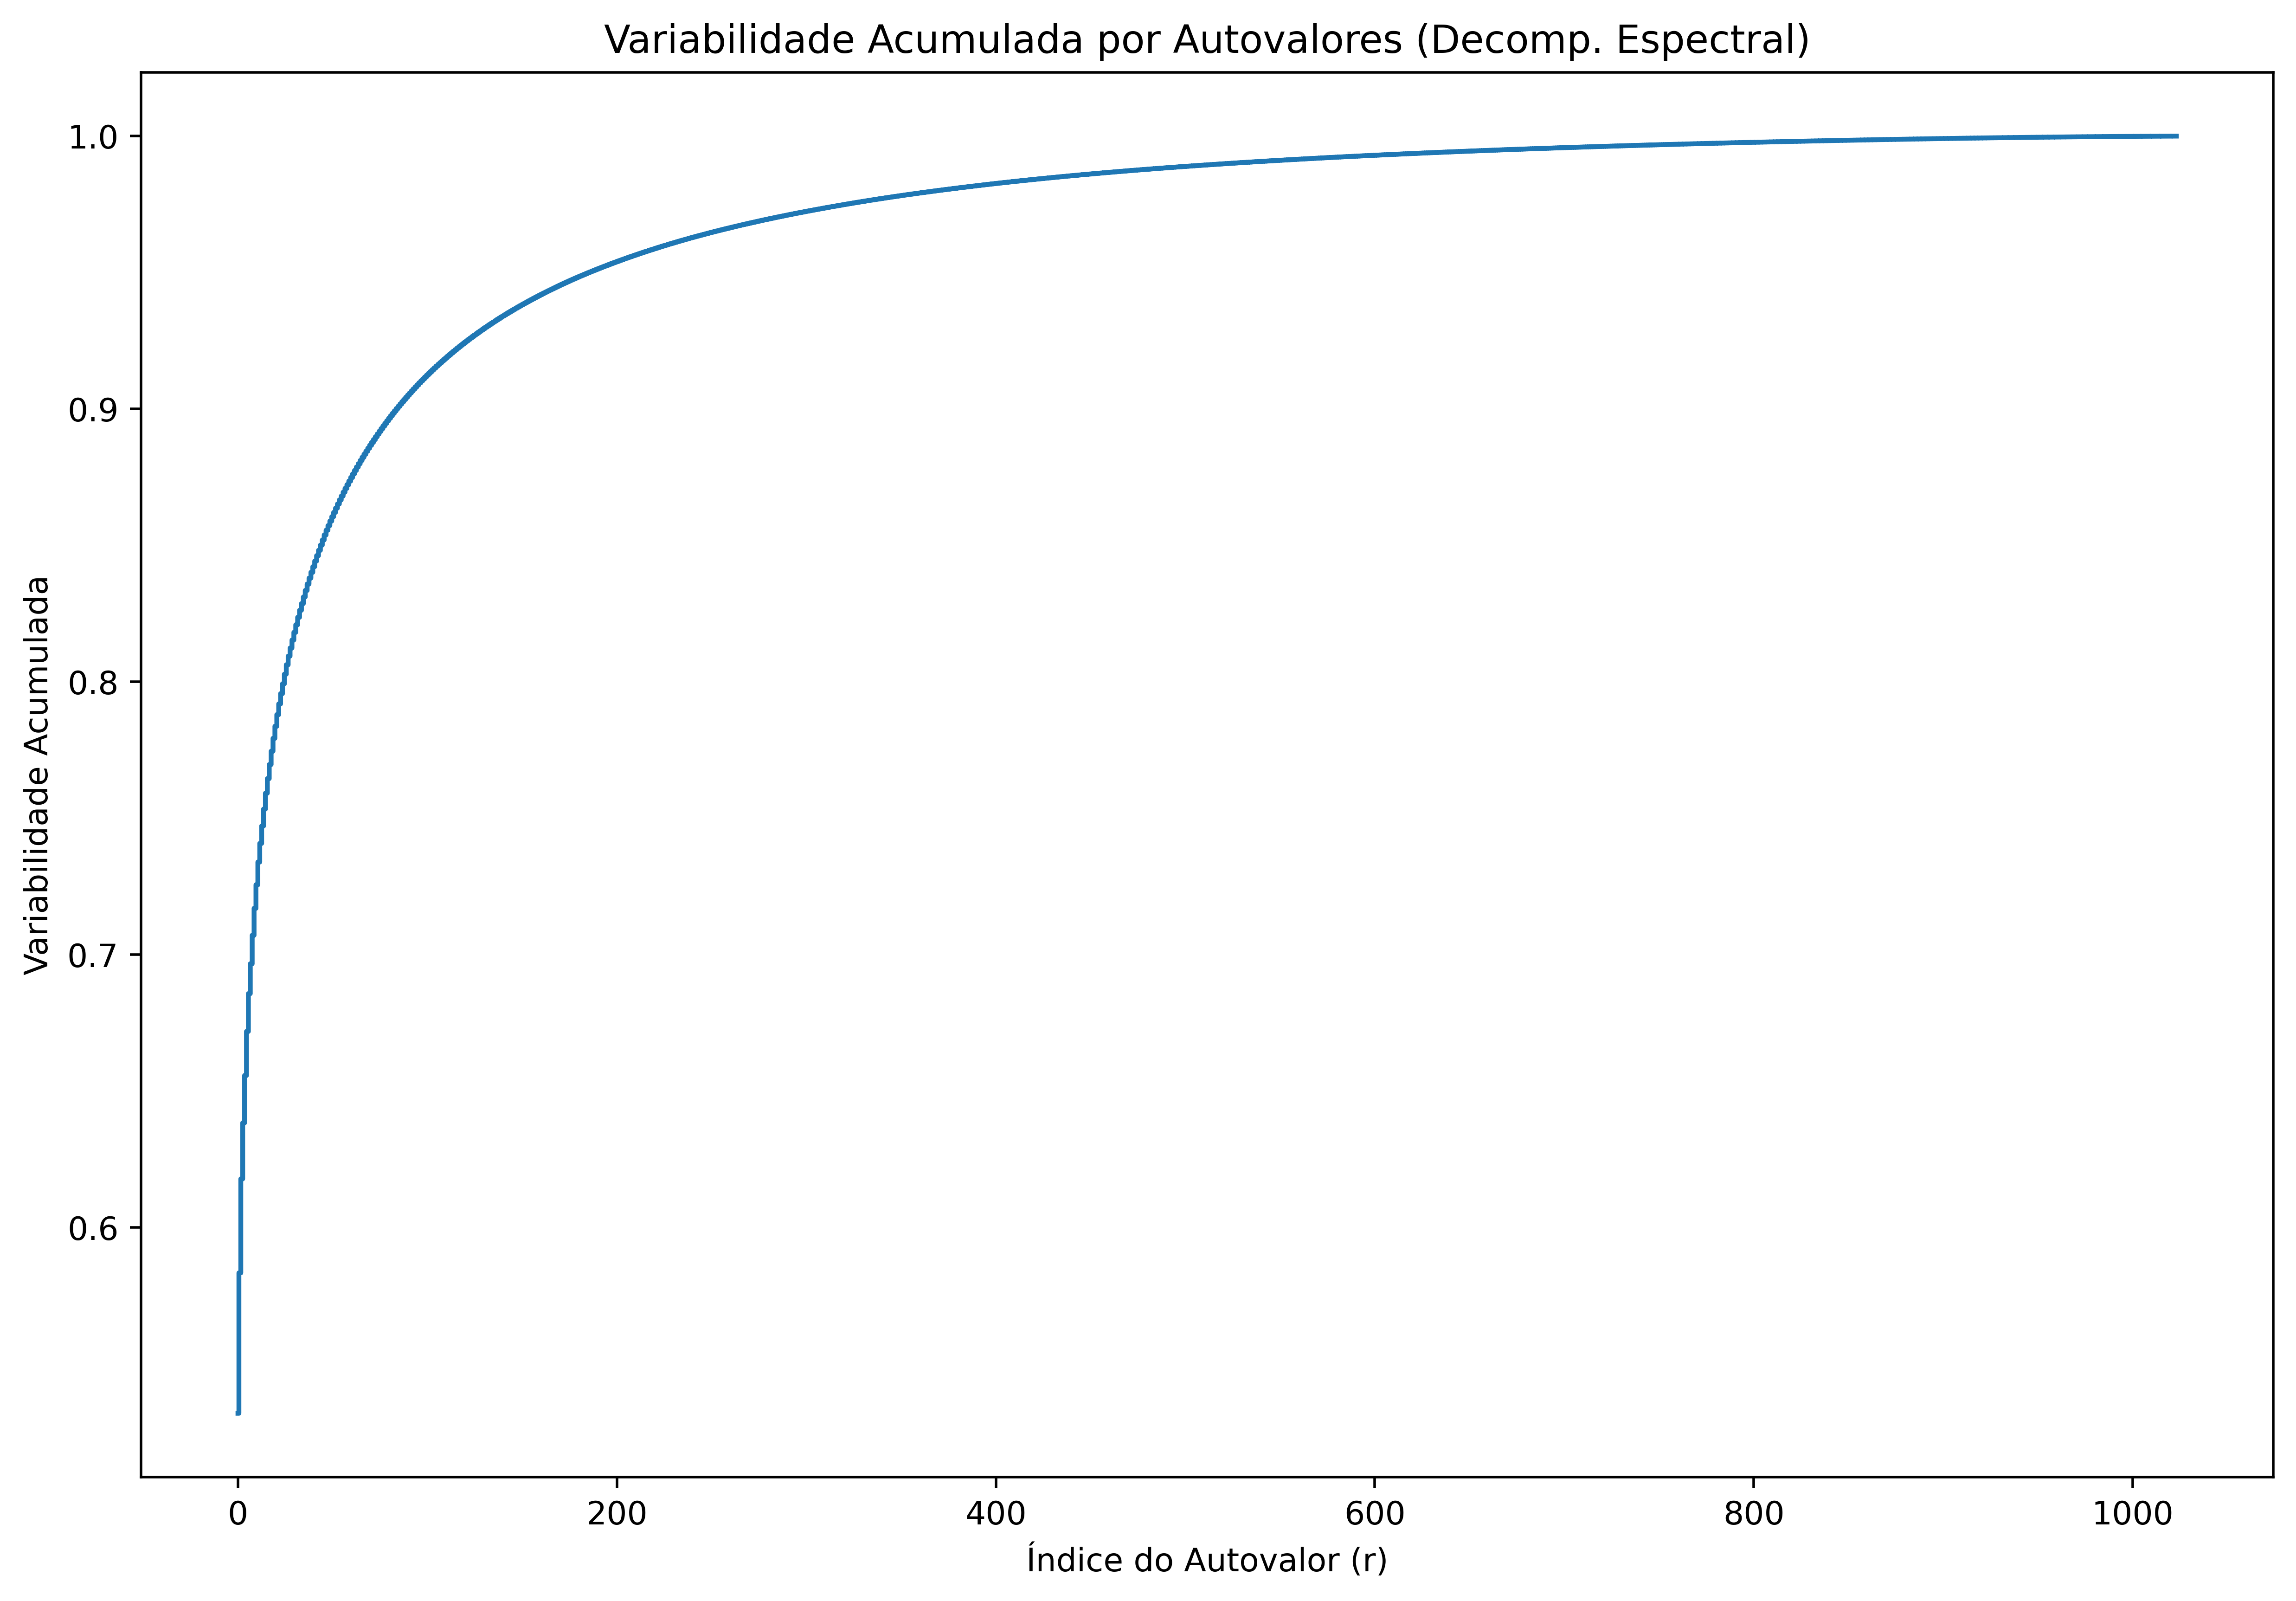
\includegraphics[width=12cm]{var_acu_espectral}
  \caption{Gráfico da variabilidade acumulada por número de autovalores na Decomposição Espectral.}
\end{figure}

Foi escolhido um valor de $95\%$ para a variabilidade acumulada e o valor de $r$ que representa esse valor é $r = 185$, como vemos na imagem a seguir.

\begin{figure}[H]
  \centering
  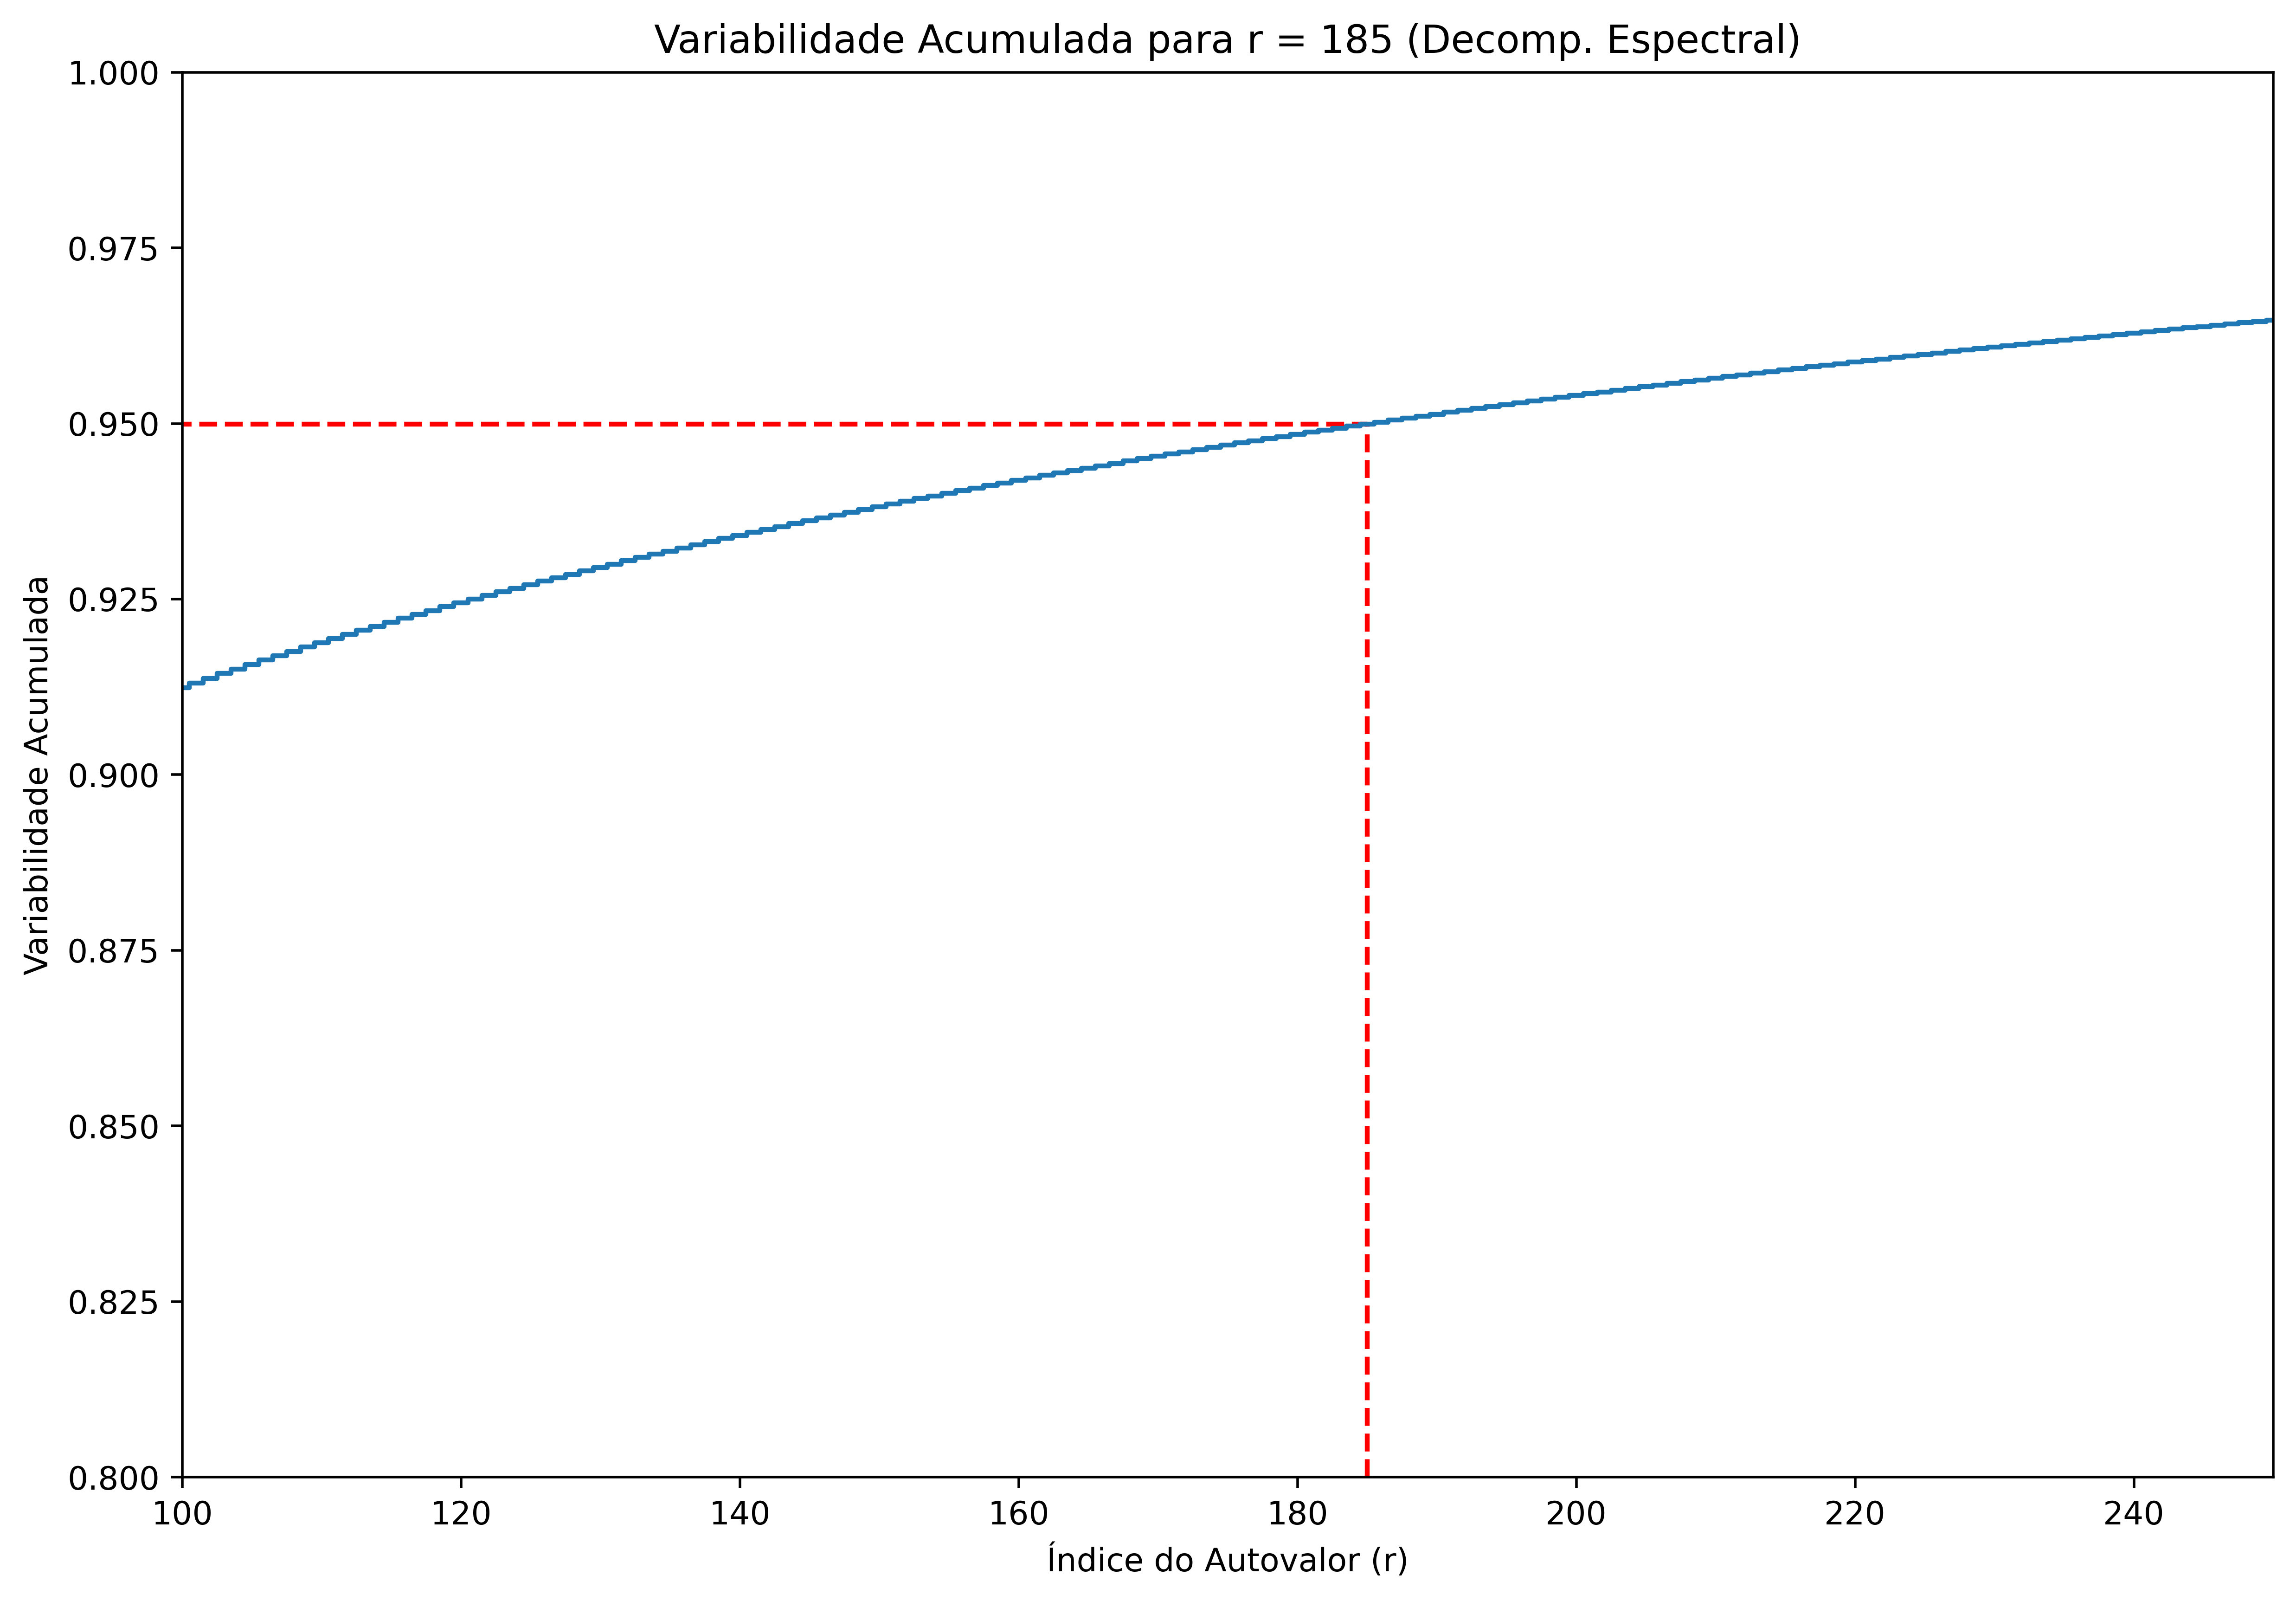
\includegraphics[width=12cm]{var_acu_espectral_185}
  \caption{Gráfico da variabilidade acumulada para 185 autovalores na Decomposição Espectral.}
\end{figure}

Com o valor de $r$ escolhido, podemos calcular a matriz $\hat{Q}$ como as $r$ primeiras colunas de $Q$ para, com isso, encontramos as componentes principais das matrizes de treino e teste, a saber

$$\hat{Z}_{train} = X_{train}\hat{Q} \text{ e } \hat{Z}_{test} = X_{test}\hat{Q}.$$

Aplicamos então o algoritmo de classificação do vizinho mais próximo (K-NN) com $k = 1$. Obtemos aqui uma acurácia de $0.7044$, para $r = 185$.

Repetimos a classificação para todos os valores de $r$ com a intenção de encontrar o que melhor se adapta aos dados em questão. Obtemos o seguinte gráfico:

\begin{figure}[H]
  \centering
  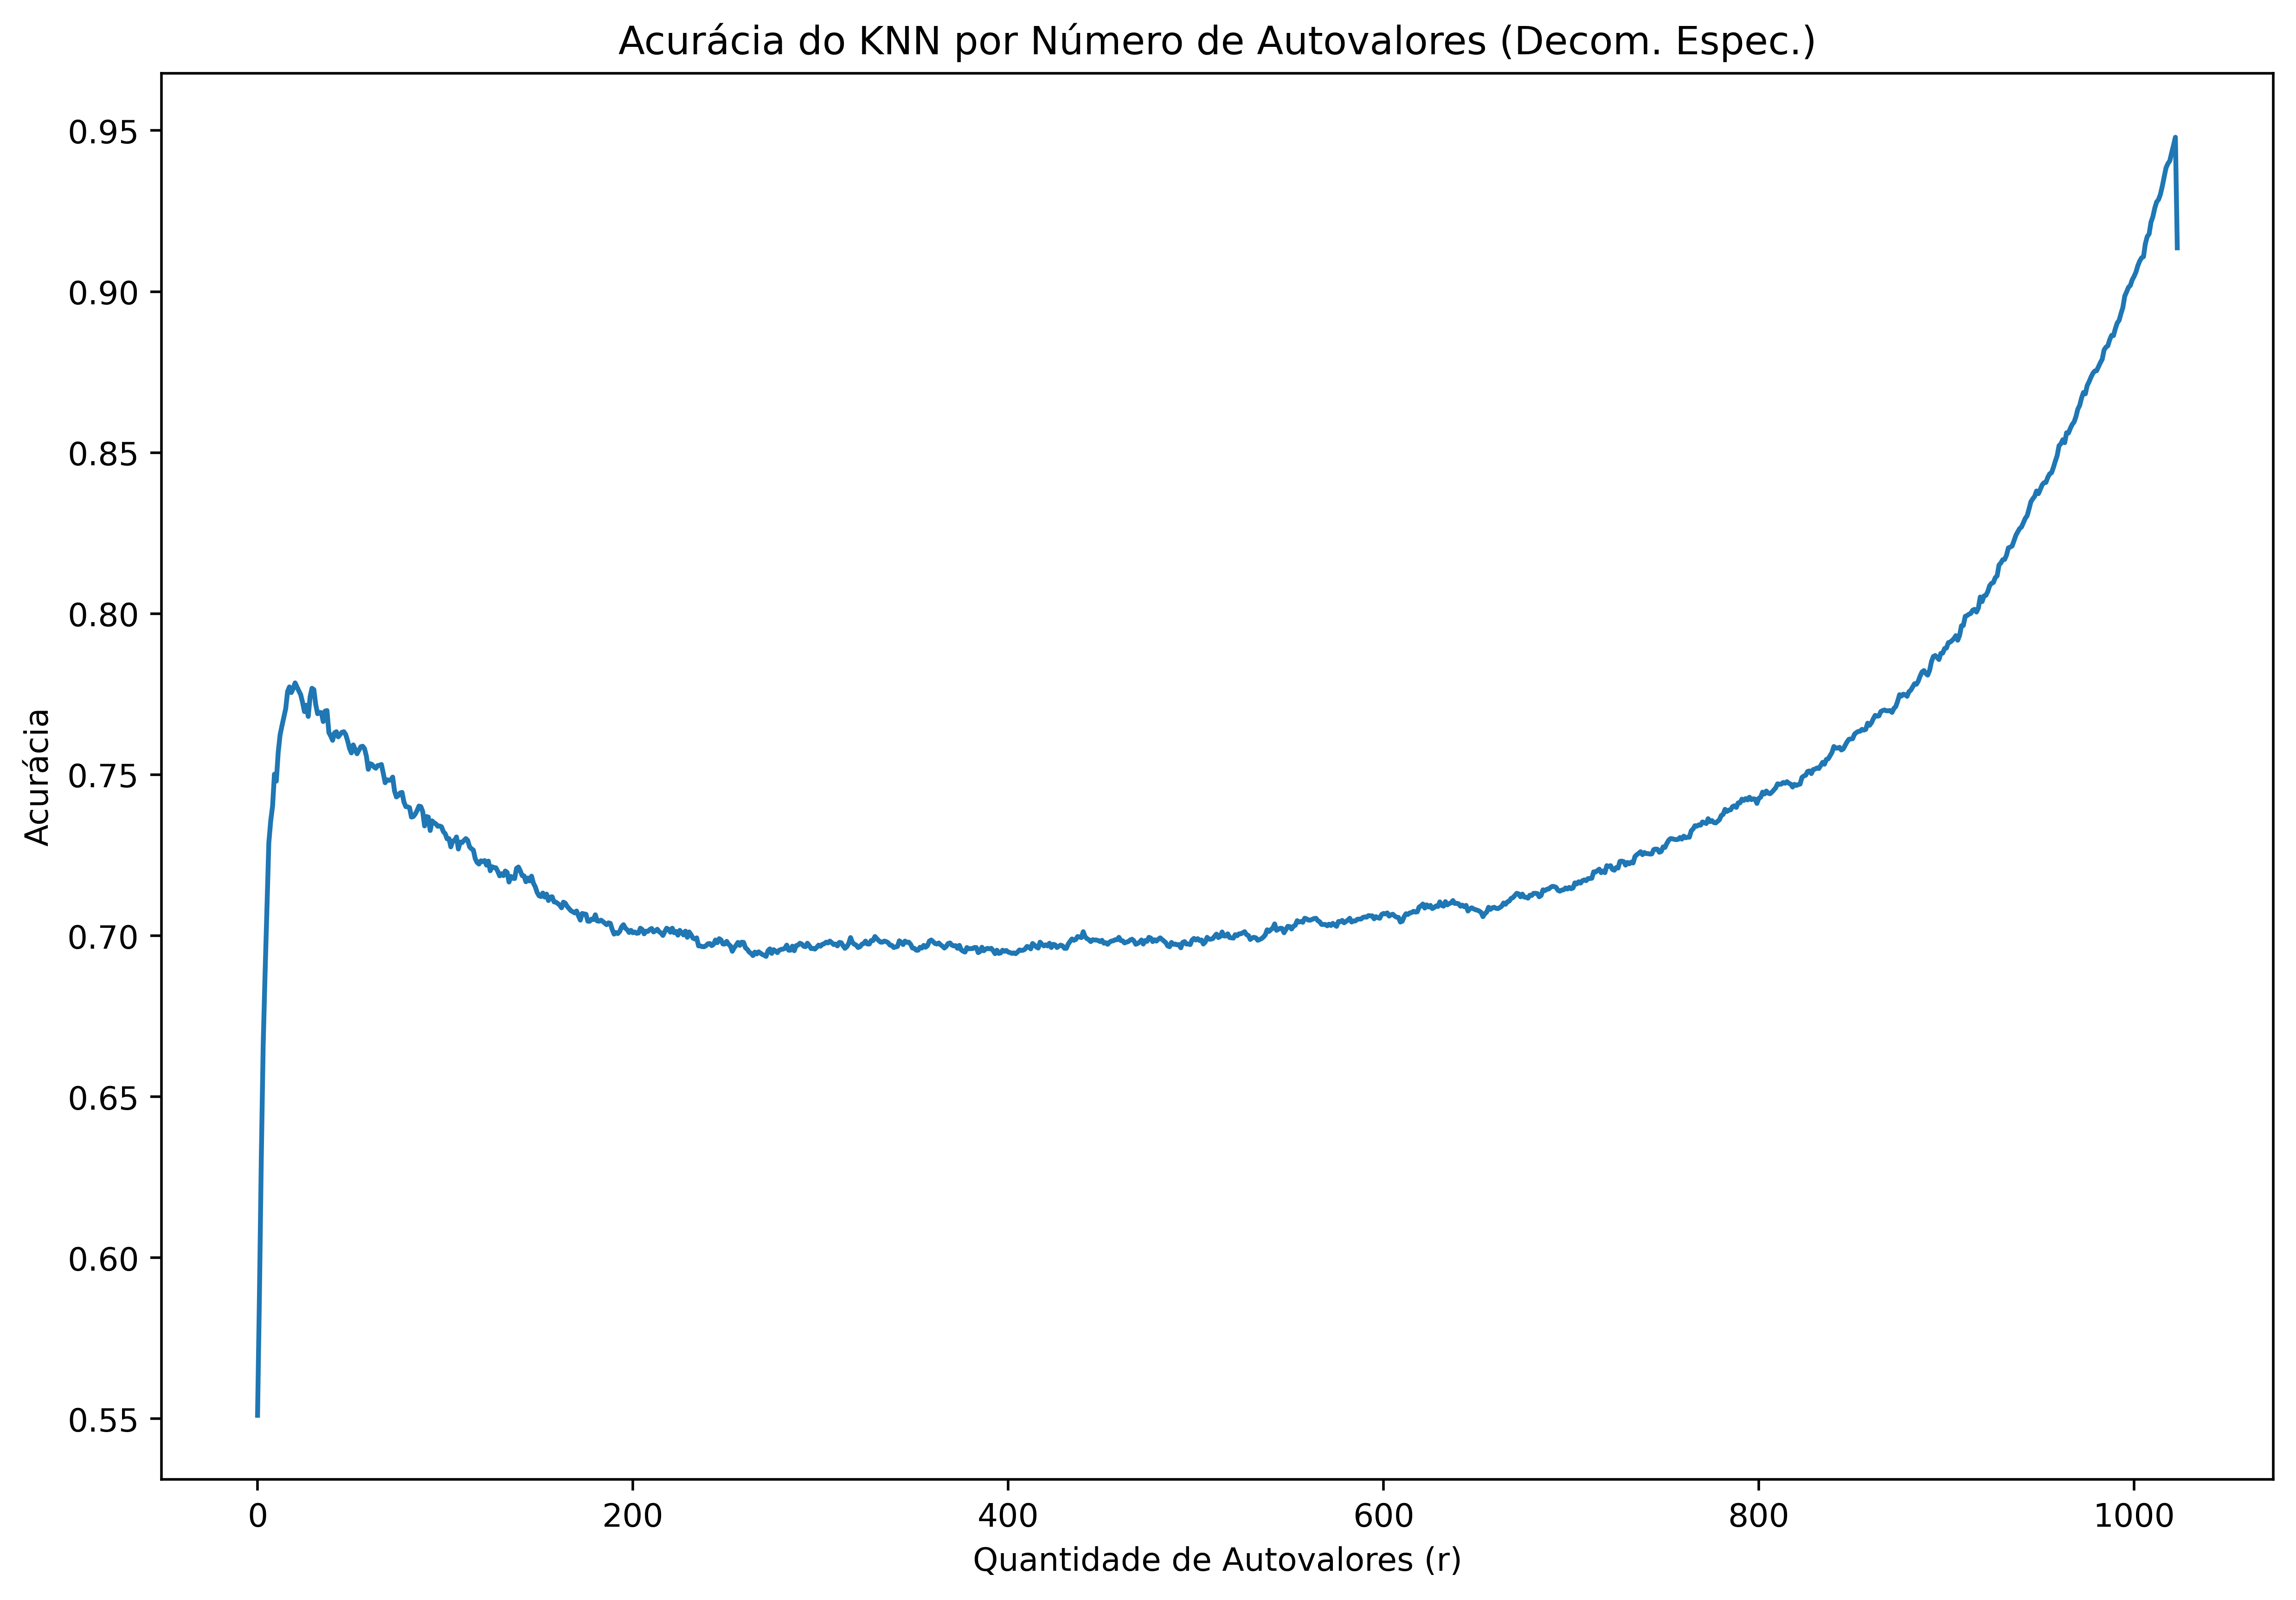
\includegraphics[width=11cm]{acuracia_espectral}
  \caption{Gráfico da acurácia do algoritmo KNN por valor de r na Decomposição Espectral.}
\end{figure}

Observamos que melhor valor de compromisso entre maior acurácia e menor $r$ corresponde a $r = 20$, como na seguinte imagem

\begin{figure}[H]
  \centering
  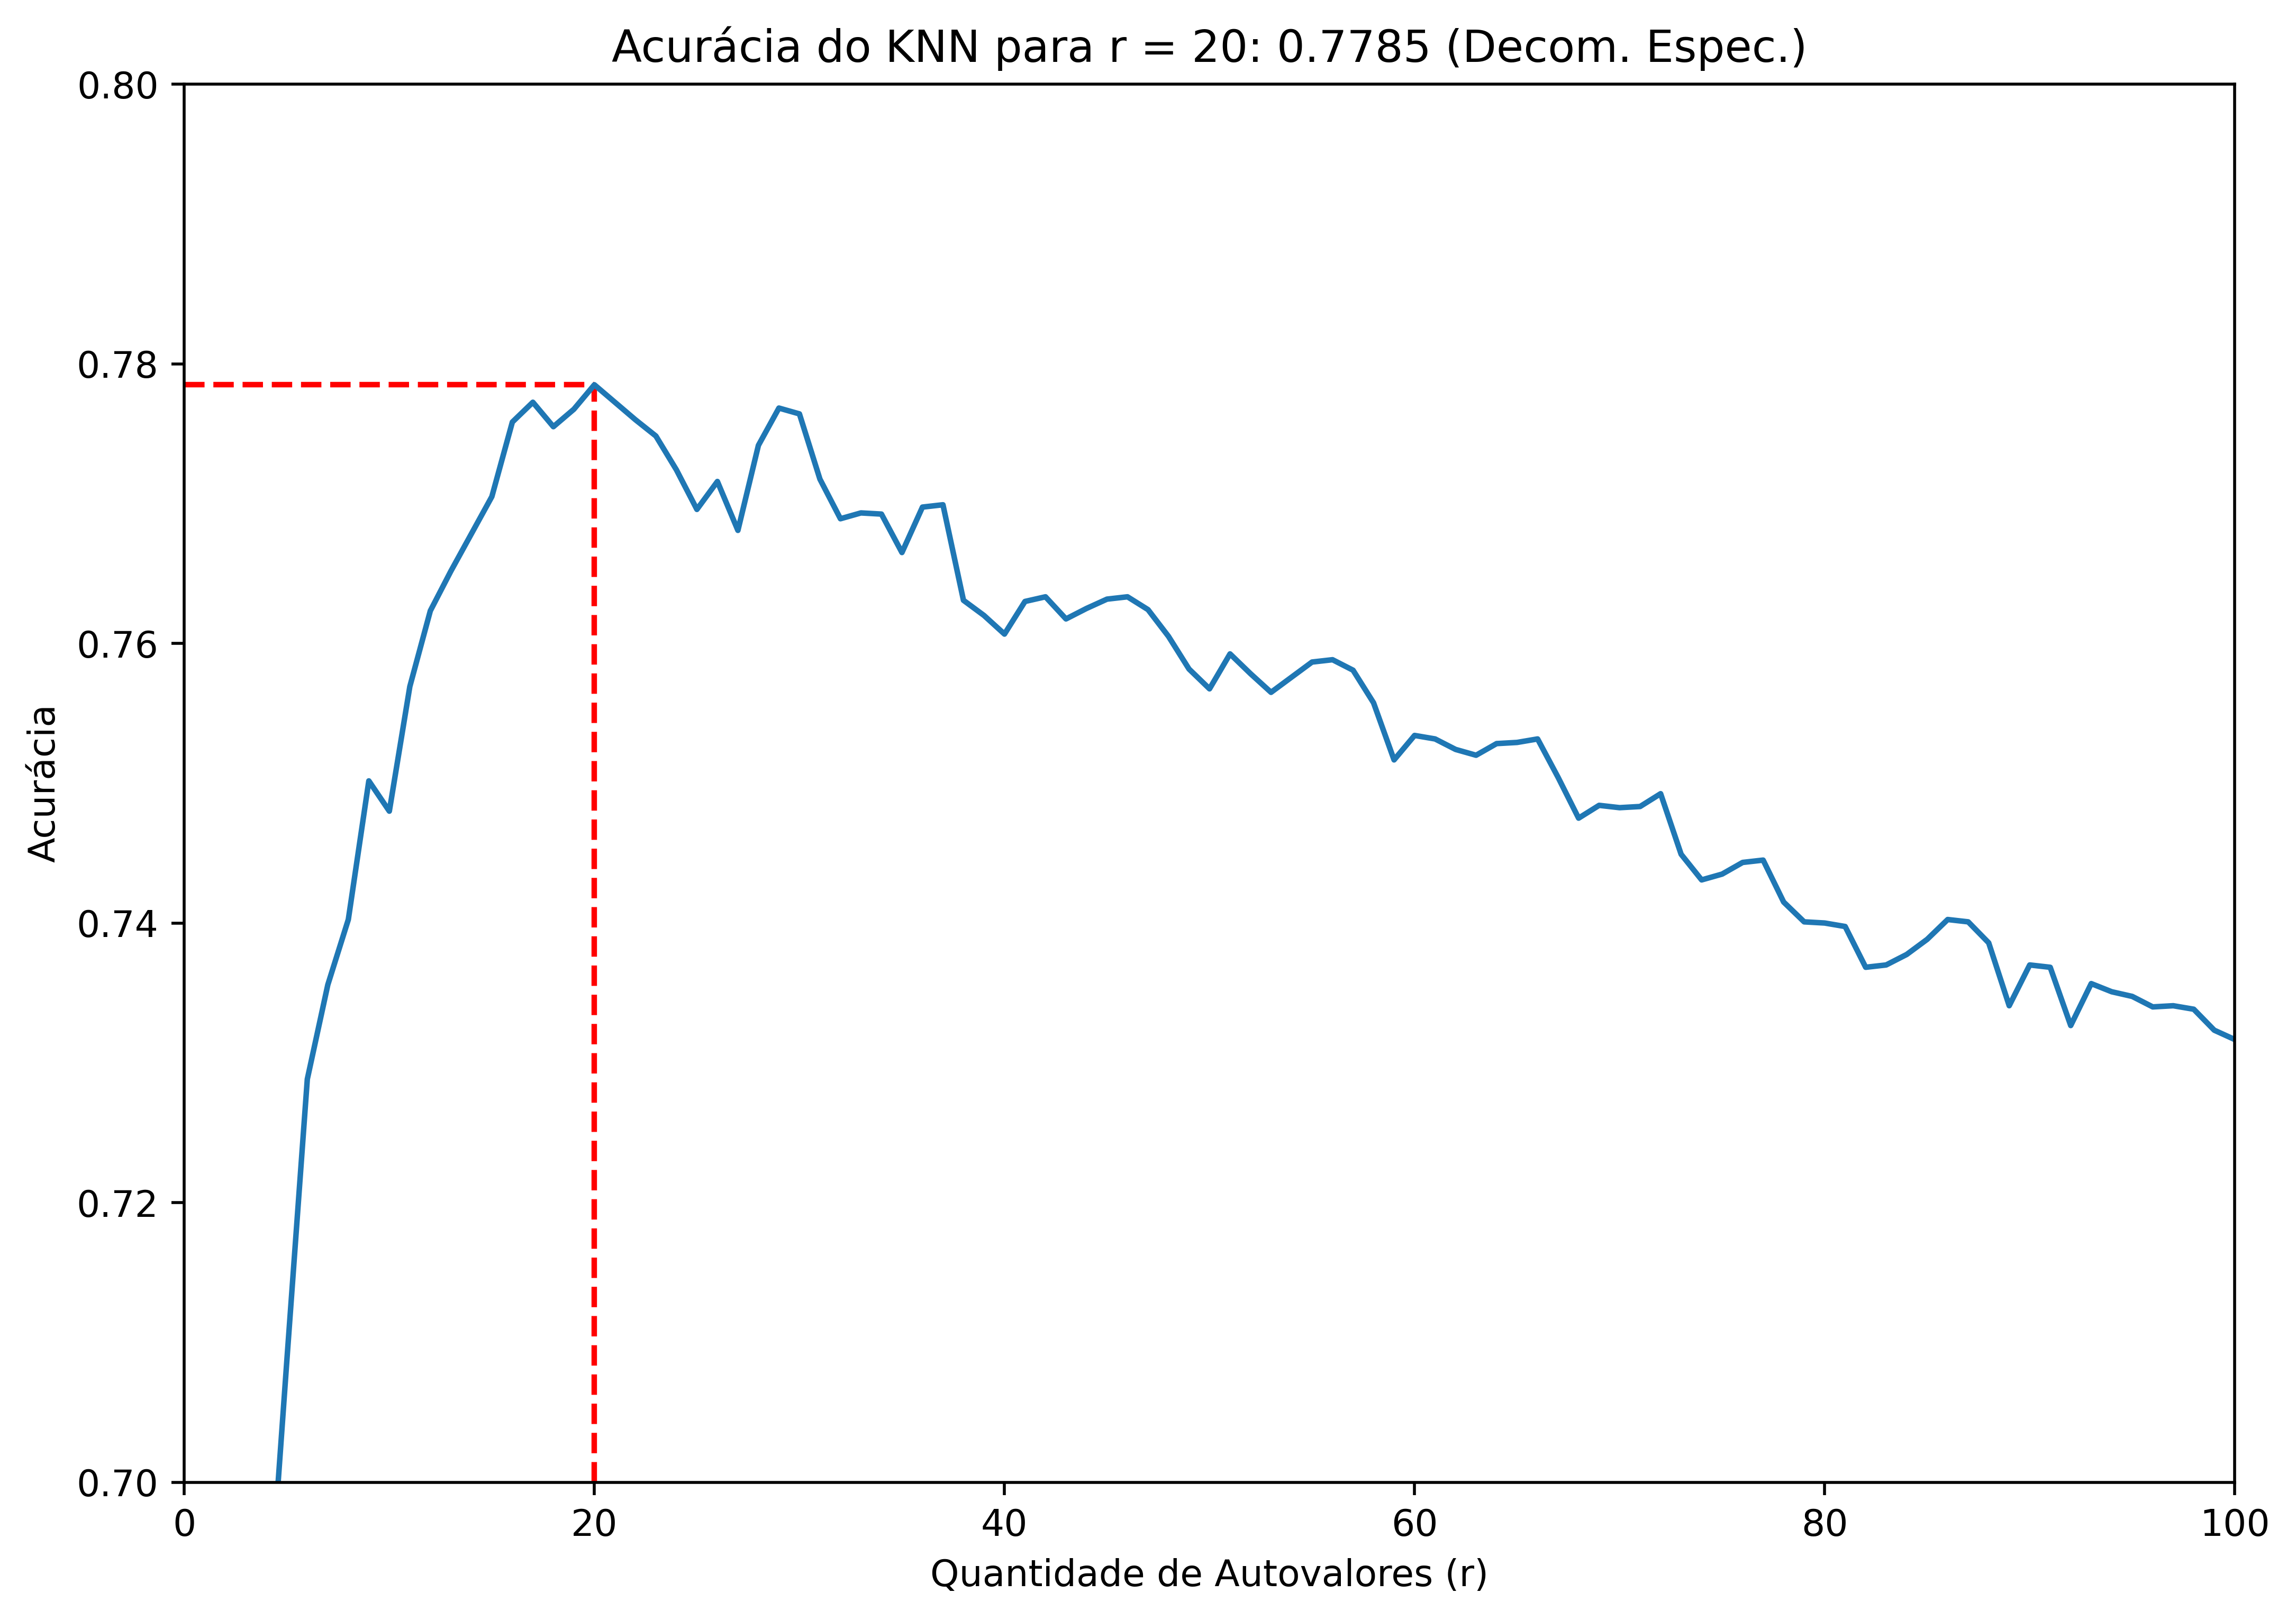
\includegraphics[width=11cm]{acuracia_espectral_20}
  \caption{Gráfico da acurácia do algoritmo KNN na Decomposição Espectral para 20 autovalores.}
\end{figure}

Assim, foi escolhido o valor de $r = 20$ e realizada novamente a classificação das imagens de teste com esse valor de $r$, obtendo, assim, uma acurácia de $0.7785$.

Resultado:\\
\textbf{
acurácia = 0.7785 para r = 20 na decomposição espectral.}

\subsection{Decomposição em Valores Singulares (SVD)}

Agora repetimos o processo, mas ao invés de utilizarmos a decomposição espectral, utilizamos a decomposição em valores singulares (SVD).

Novamente lemos os dados e obtemos 4 matrizes: \textit{X\_train, y\_train, X\_test, y\_test}, com \textit{X\_train} e \textit{X\_test} já centralizadas.

Calculamos a SVD reduzida da matriz \textit{X\_train}, correspondente aos dados de treinamento

$$X\_train = USV^T$$

com a função \pyth{np.linalg.svd(X_train, full_matrices=False)}. Aqui o parâmetro \pyth{full_matrices} deve ser \pyth{False} pois queremos a SVD reduzida. Isso nos retorna as matrizes $U$, $S$ e $V^T$. Os valores singulares já são retornados em ordem decrescente em $S$, de acordo com a documentação do \textit{NumPy}.

Ao visualizarmos o gráfico da variabilidade acumulada utilizando a SVD, obtemos

\begin{figure}[H]
  \centering
  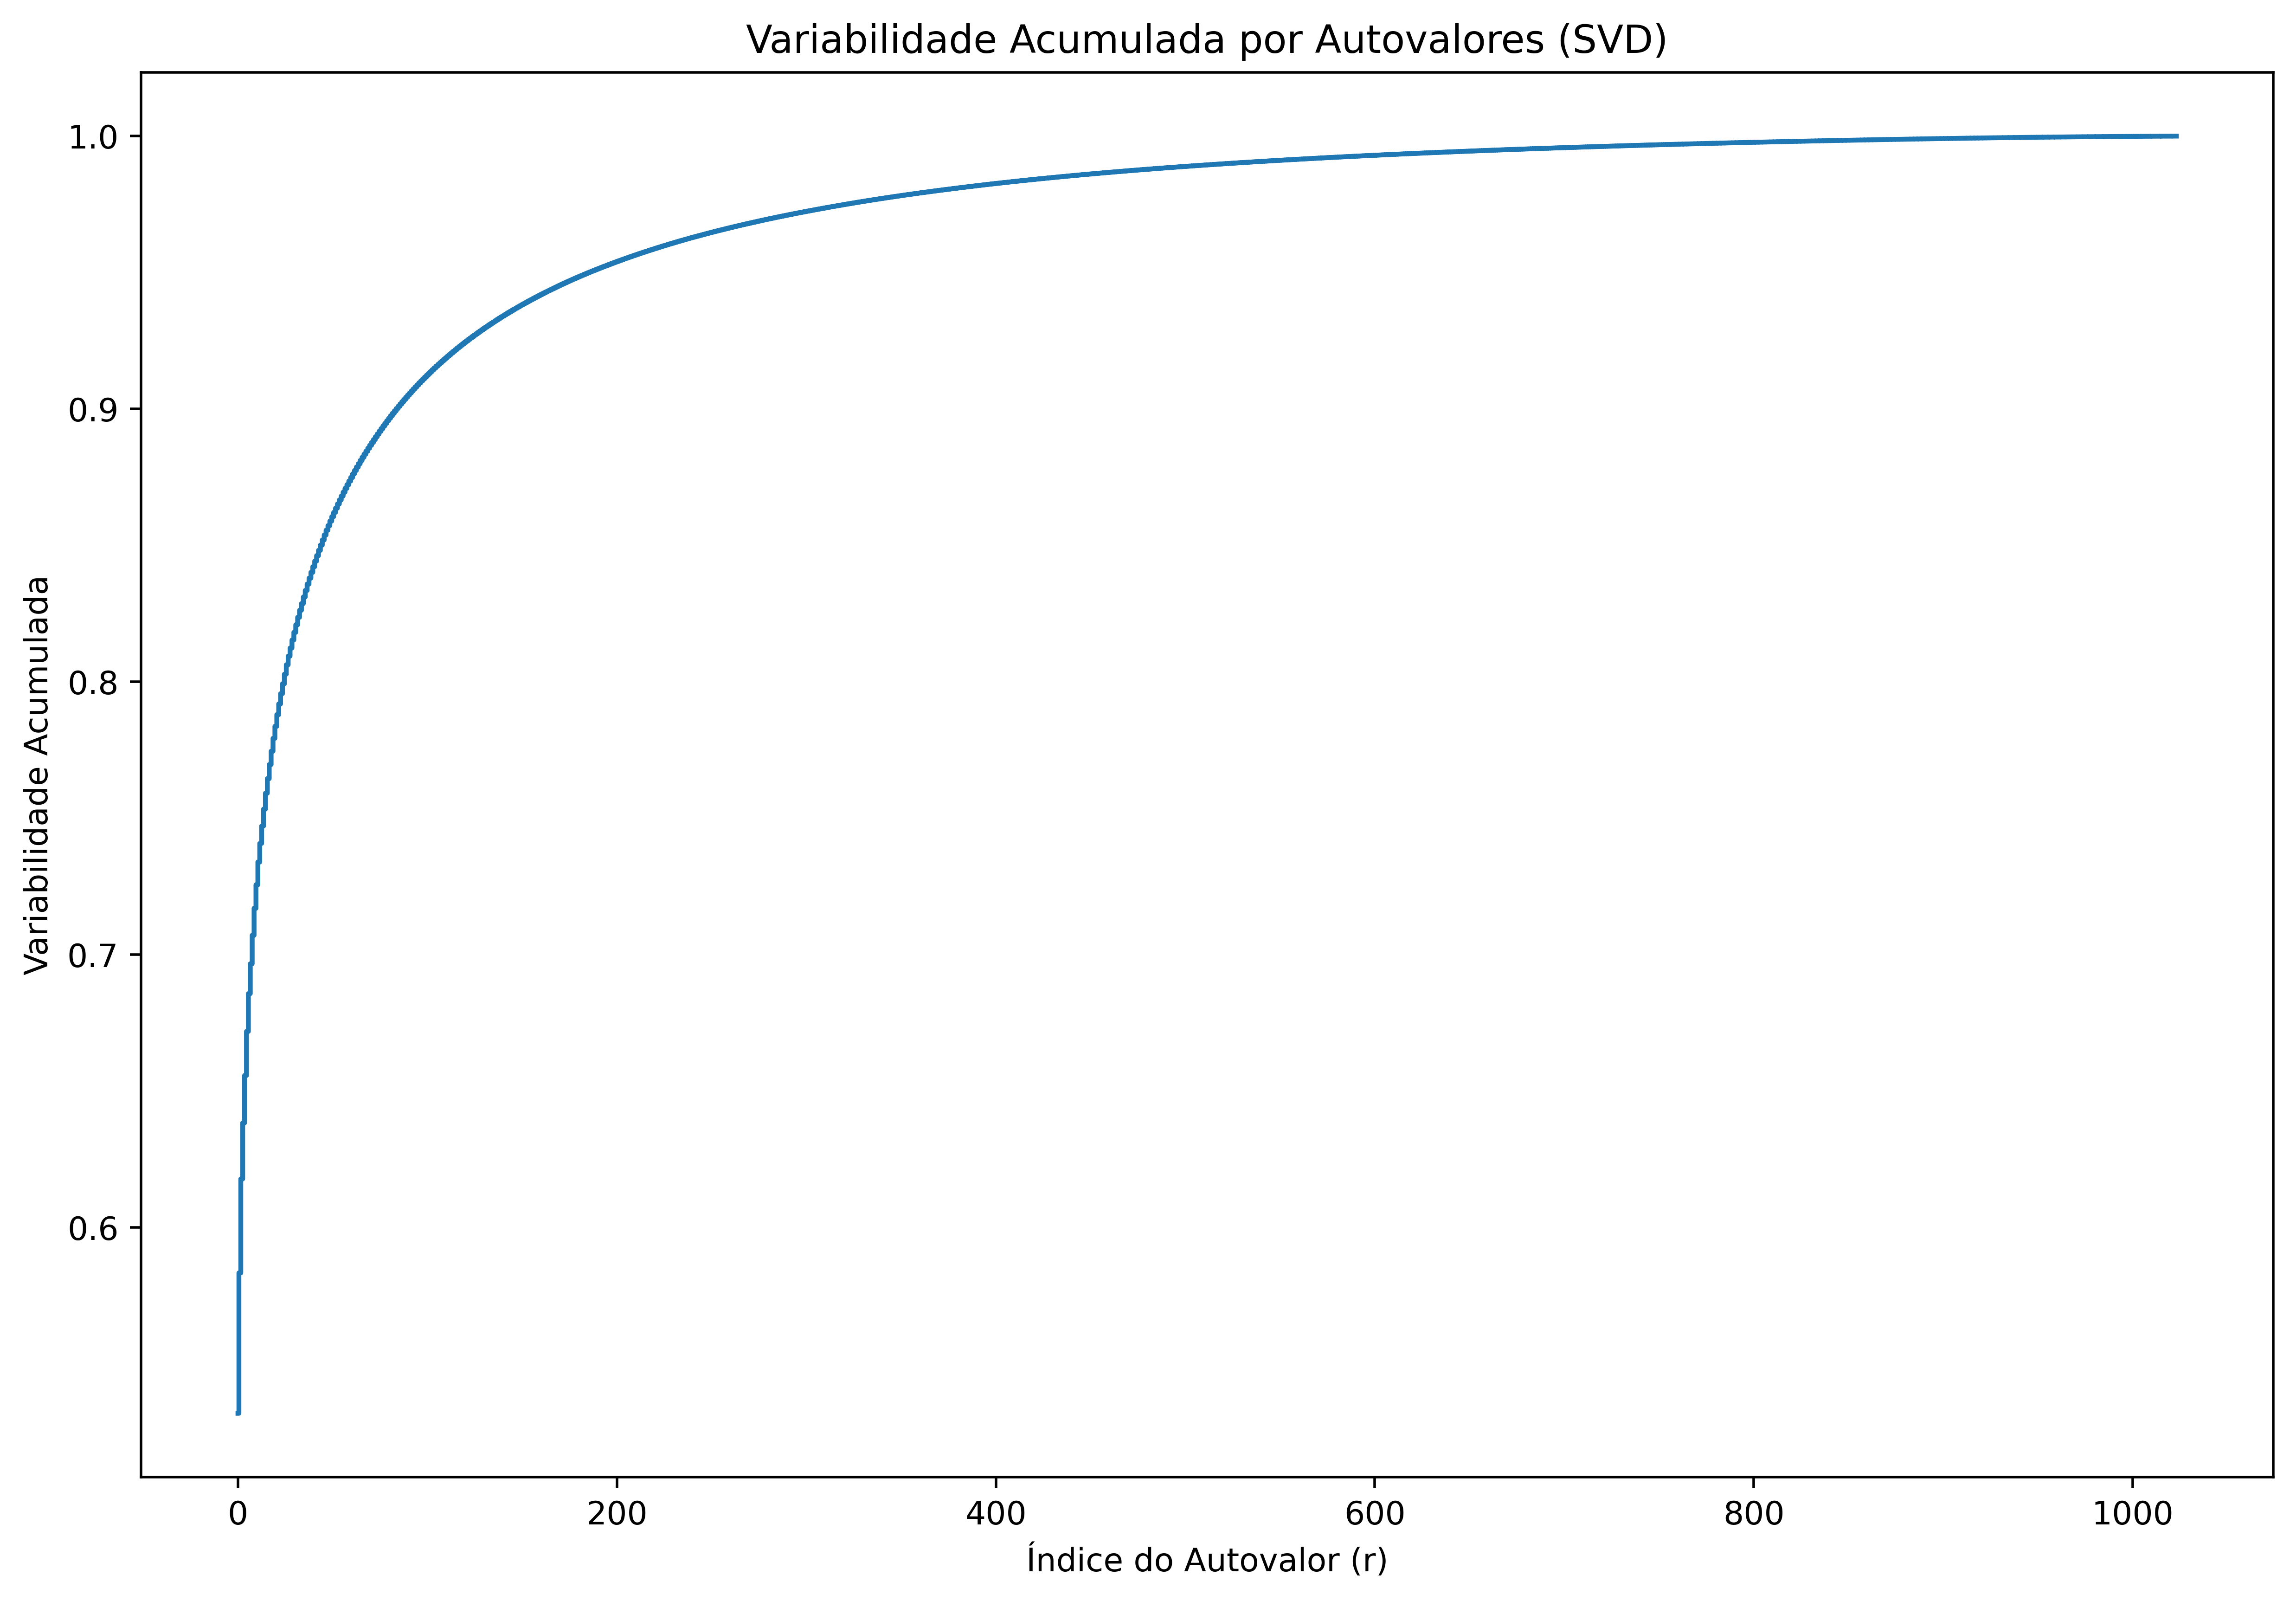
\includegraphics[width=10cm]{var_acu_svd}
  \caption{Gráfico da variabilidade acumulada por número de autovalores na SVD.}
\end{figure}

Lembrando que aqui a variabilidade acumulada foi calculada com o quadrado dos $\sigma_i$'s, para obtermos os $\lambda_i$'s.

Novamente foi utilizado um valor de $95\%$ para a variabilidade acumulada, o que corresponde a $r = 185$, como mostra a figura a seguir

\begin{figure}[H]
  \centering
  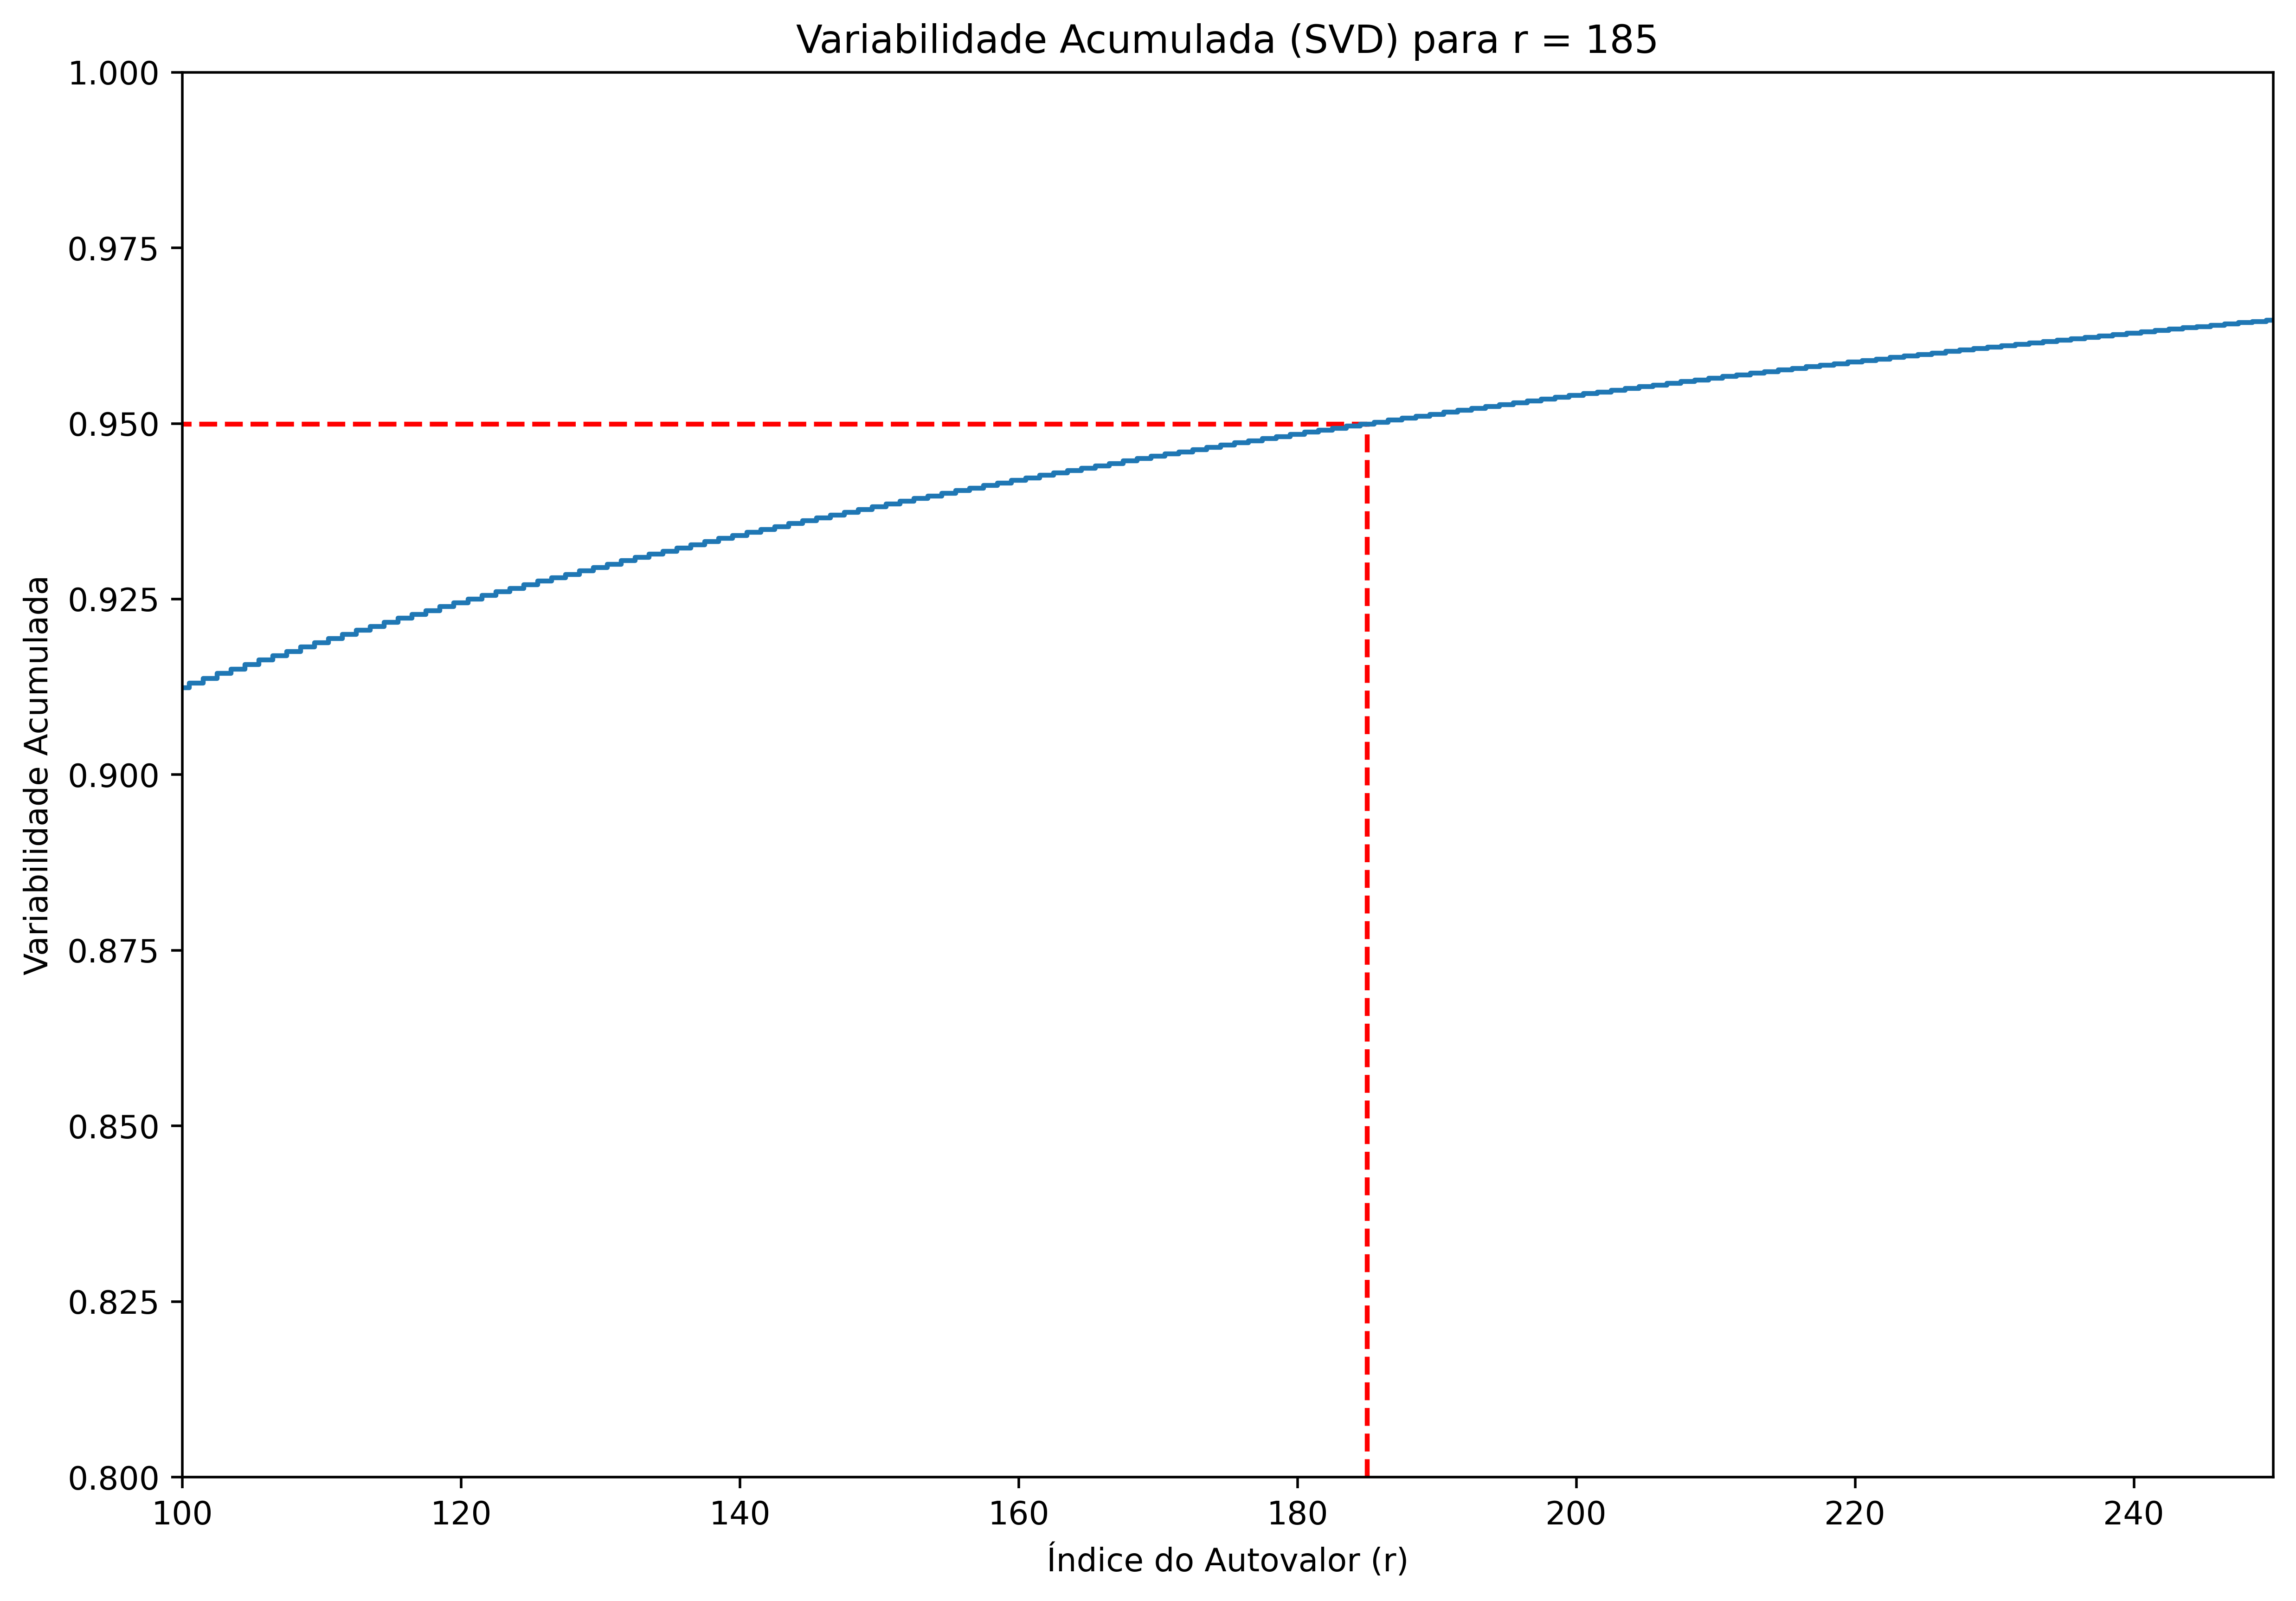
\includegraphics[width=12cm]{var_acu_svd_185}
  \caption{Gráfico da variabilidade acumulada para 185 autovalores na SVD.}
\end{figure}

Com o valor de $r$ já definido, encontramos a matriz $V_r$ cujas colunas são as $r$ primeiras colunas de $V$, nesse caso, as 185 primeiras colunas de $V$.

Calculamos então as componentes principais utilizando $V_r$ para obter

$$\hat{Z}_{train} = X_{train}\hat{V} \text{ e } \hat{Z}_{test} = X_{test}\hat{V}.$$

Finalmente, realizamos novamente a classificação das imagens utilizando o algoritmo KNN com $k = 1$, agora com as componentes principais da SVD. Obtemos os seguinte gráfico da acurácia por valor de r

\begin{figure}[H]
  \centering
  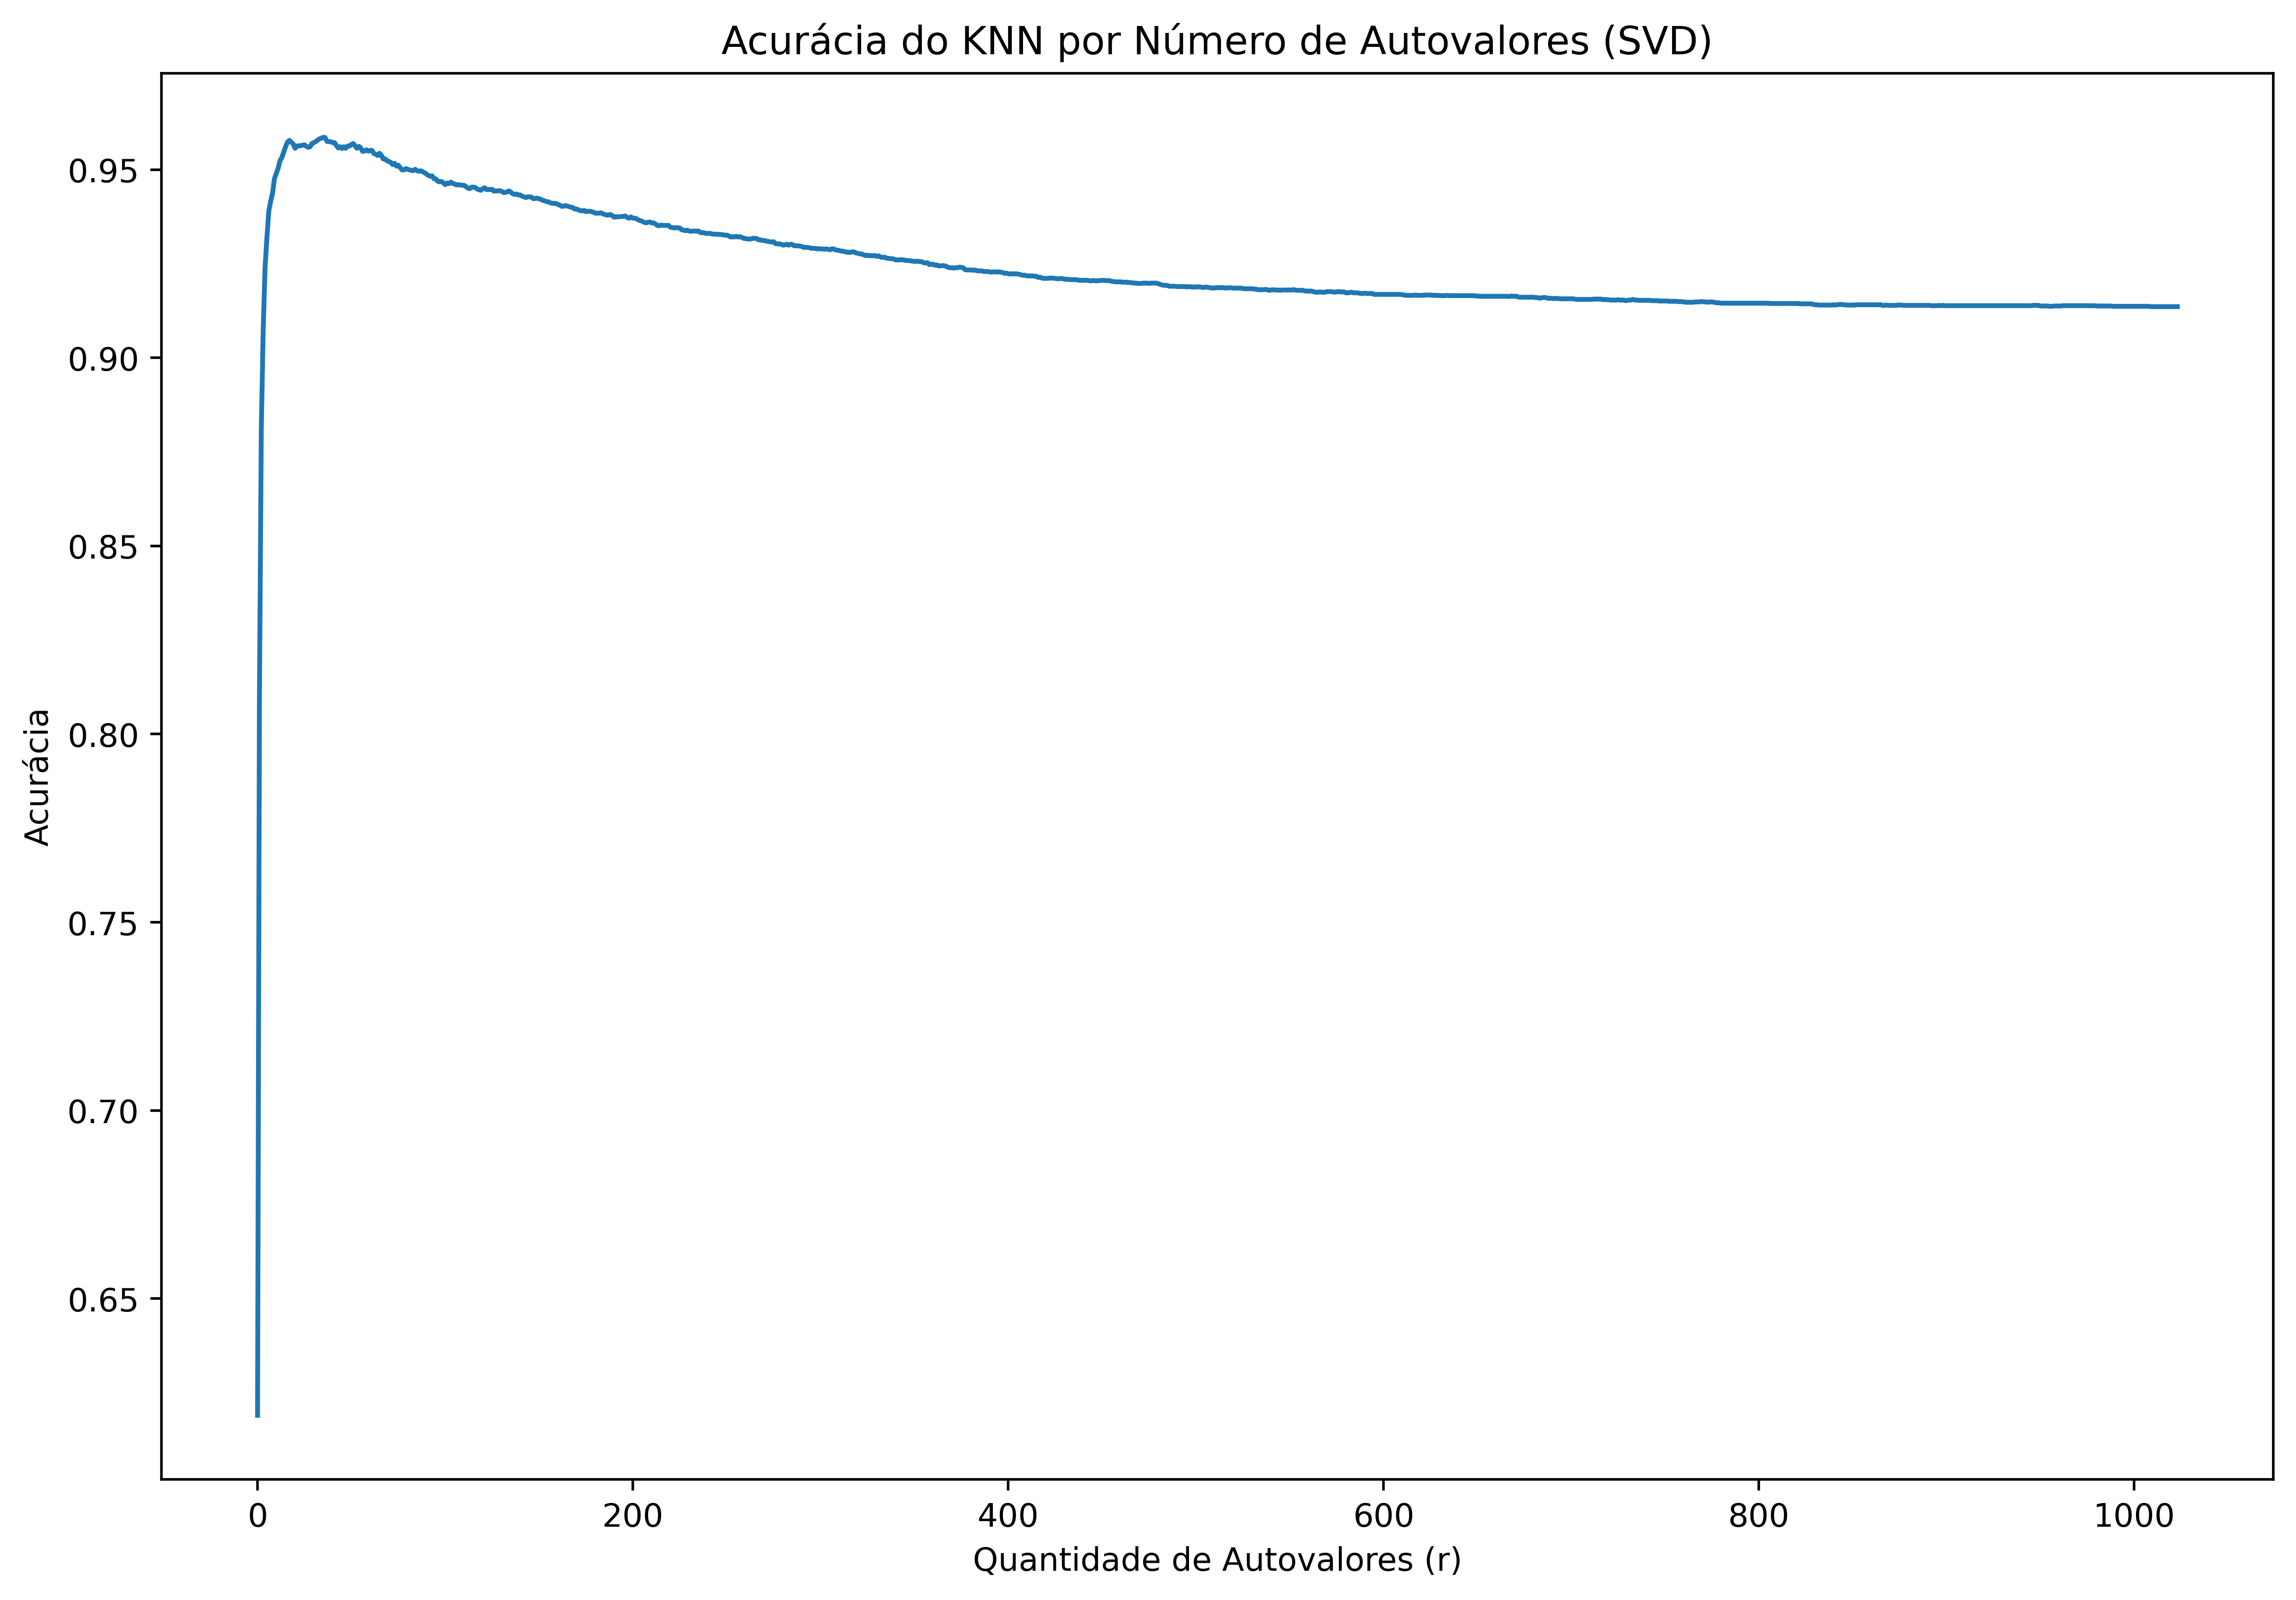
\includegraphics[width=11.5cm]{acuracia_svd}
  \caption{Gráfico da acurácia do algoritmo KNN por valor de r na SVD.}
\end{figure}

Observamos que melhor valor com maior acurácia e menor $r$ corresponde a $r = 17$, como na seguinte imagem

\begin{figure}[H]
  \centering
  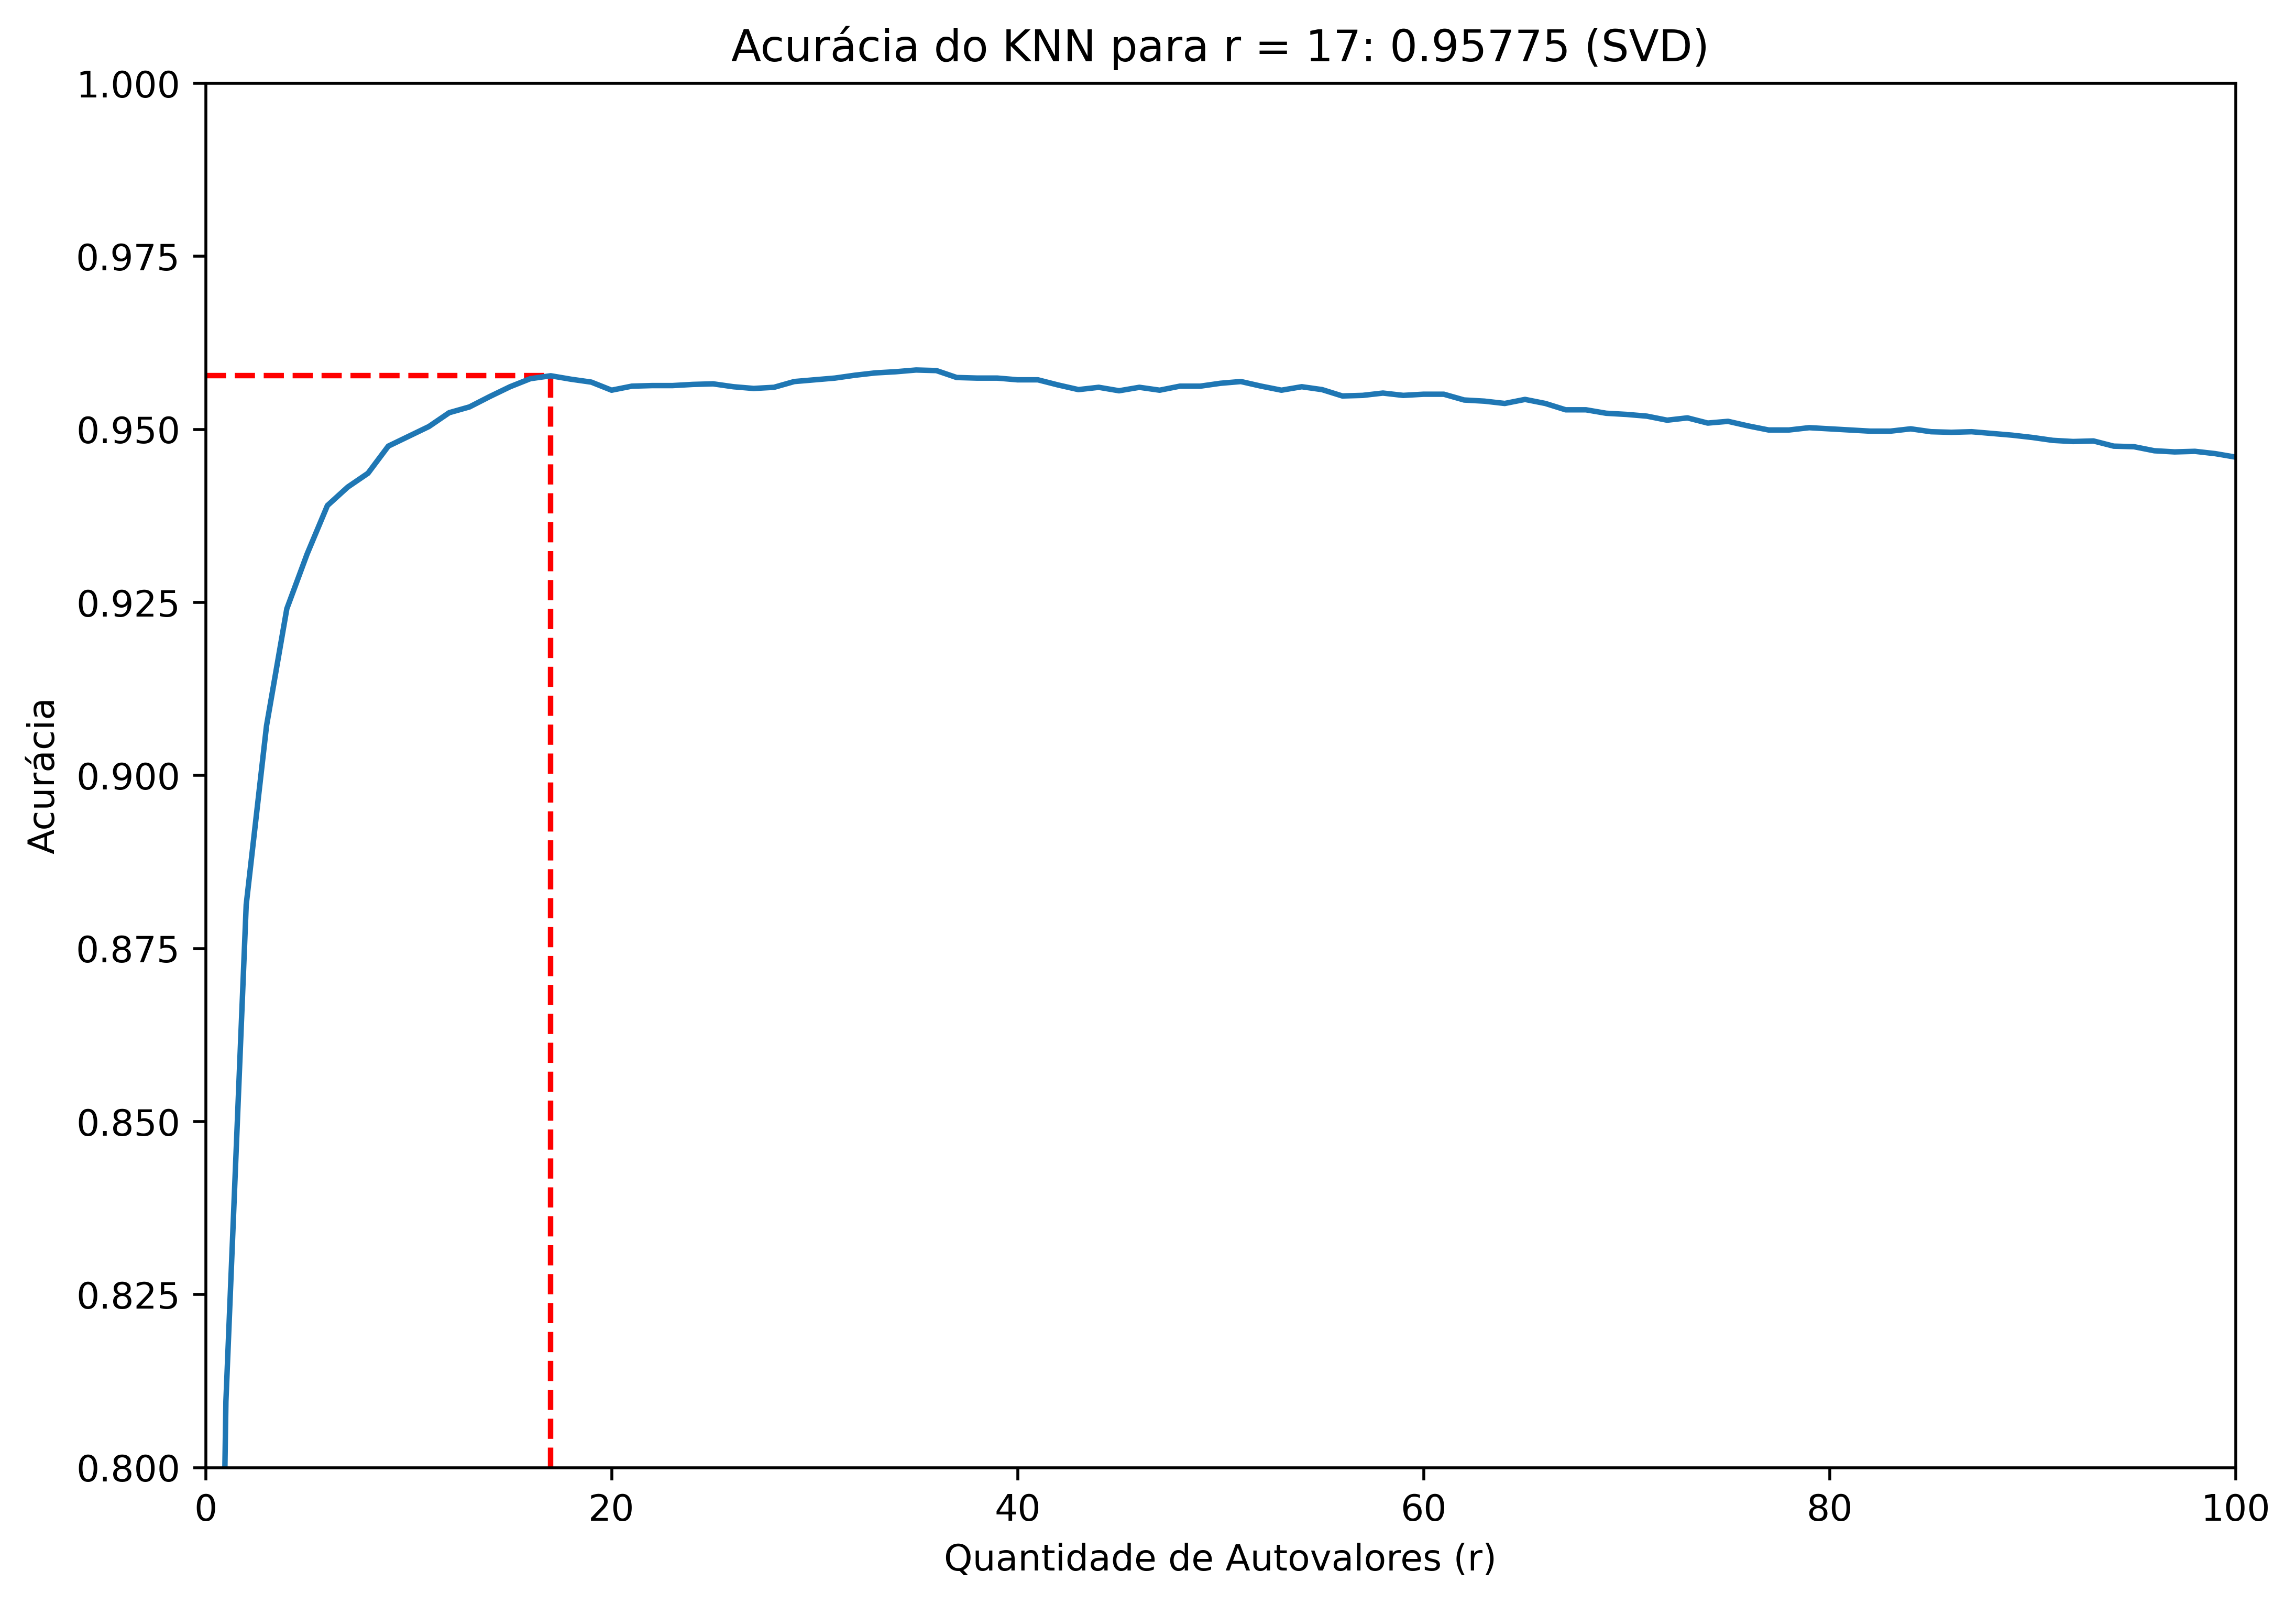
\includegraphics[width=11.5cm]{acuracia_svd_17}
  \caption{Gráfico da acurácia do algoritmo KNN para 17 autovalores na SVD.}
\end{figure}

Assim, foi escolhido o valor de $r = 17$ e realizada novamente a classificação das imagens de teste com esse valor de $r$, obtendo, assim, uma acurácia de $0.9577$.

Resultado:\\
\textbf{
acurácia = 0.9577 para r = 17 na SVD.}

Notamos que o valor de acurácia utilizando as componentes principais advindas da SVD é bem maior que a acurácia utilizando as componentes principais provenientes da decomposição espectral.

\newpage

\section{Conclusão}

O problema de classificar imagens utilizando algoritmos como o de vizinhos mais próximos (KNN, com $k = 1$) esbarra na quantidade elevada de características que existem nas imagens. Em uma imagem de baixa resolução de apenas 32 pixels, temos 1024 características para cada imagem.

Para contornar esse problema, vimos como realizar a redução de dimensionalidade dos dados, utilizando duas técnicas: a Decomposição Espectral e a Decomposição em Valores Singulares (SVD). Assim, conseguimos obter, ao utilizar a SVD, uma acurácia de $95,77\%$ para os dados de teste utilizando apenas 17 das 1024 características.

\newpage
\section{Trabalhos Futuros}

Atingir maiores acurácias com algoritmos mais avançados e utilizar diferentes problemas para serem classificados são possíveis rumos a serem tomados em futuros trabalhos.

\newpage
\section{Referências Bibliográficas}

\nocite{algebra-linear-teoria-e-aplicacoes}

\printbibliography[heading=none]




\end{document}